\documentclass[12pt,a4paper,titlepage,final, svgnames, twoside, openright]{book}
\author{Carlos Vázquez Sánchez}

\usepackage[utf8]{inputenc}
\usepackage[T1]{fontenc}
\usepackage{lmodern}
\usepackage{amsmath}
\usepackage{amsfonts}
\usepackage{amssymb}
\usepackage{makeidx}
\usepackage{graphicx}
\usepackage{tikz}
\usetikzlibrary{arrows}
\usepackage[colorlinks=true,linkcolor=black,urlcolor=blue]{hyperref} 
\usepackage[spanish]{babel}
\usepackage{url}
\usepackage{color}
\setlength{\textwidth}{125mm}
\setlength{\textheight}{195mm}
\setlength{\oddsidemargin}{6mm}
\setlength{\evensidemargin}{28mm}
\setlength{\topmargin}{-5mm}
\usepackage{longtable}
\usepackage{ltxtable} 

\addto\captionsspanish{\renewcommand{\figurename}{Figura}}

\renewcommand*{\figureautorefname}{figura}
\renewcommand*{\tableautorefname}{tabla}
\renewcommand*{\chapterautorefname}{capítulo}

\usepackage{lscape}
\usetikzlibrary{babel}
\usepackage[]{algorithm2e}

\usepackage{color}
\usepackage{float}
\usepackage[left=3cm,right=2cm, bottom=4cm]{geometry}

\usepackage{fancybox}
\usepackage{caption}
\usepackage{subcaption}
\usepackage{times}
\usepackage{verbatim}
\usetikzlibrary{arrows,shapes,positioning}
\usepackage{emptypage} % Para eliminar encabezado de las páginas en blanco
\usepackage{chngcntr}
\usepackage{etoolbox}
\usepackage{listings}
\usepackage{standalone}
\hypersetup{
	colorlinks,
	citecolor=Black,
}
\usepackage{fancyhdr}
\setlength{\unitlength}{1 cm} %Especificar unidad de trabajo
\thispagestyle{empty}
\begin{figure}[htb]
\begin{center}

\includegraphics[width=4cm]{./imagenes/logoURJC}
\end{center}
\end{figure}
\begin{center}
\textbf{{\Huge Universidad Rey Juan Carlos}\\[0.5cm]
{\LARGE Escuela Técnica Superior Ingeniería Informática}}\\[1.25cm]
{\Large XXXXXX XXXX}\\[2.3cm]
{\LARGE \textbf{TFG}}\\[3cm]
{\large GIS - Carlos Vázquez Sánchez}\\[1cm]
Móstoles - \today
\end{center}



\begin{document}
	\portada{Desarrollo e implementación de algoritmos heurísticos para la gestión óptima de flujo en tráfico aéreo}{Ingeniería del Software}{Curso 2016--2017}{Carlos Vázquez Sánchez}{Antonio Alonso Ayuso}

	
	\newpage
	\tableofcontents
	\listoffigures

	\chapter{Introducción y nuevos objetivos}

\section{Introducción}
El número de pasajeros de avión en las últimas décadas ha aumentado exponencialmente, conllevando un aumento prácticamente similar en el tráfico aéreo. Tan sólo España tuvo el año 2012 195 millones de viajeros en la red AENA, con el aeropuerto de Madrid-Barajas 45 millones de viajeros, y el de Barcelona-El Prat 35 millones. \\
Este rápido aumento del número de aviones en el espacio aéreo, actualmente 11.000 de media por minuto, sumado a las limitaciones estructurales que tienen los aeropuertos para expenderse, ha ocasionado un importante problema de sobresaturación.
\begin{figure}[H]
	\begin{center}
		\centering
		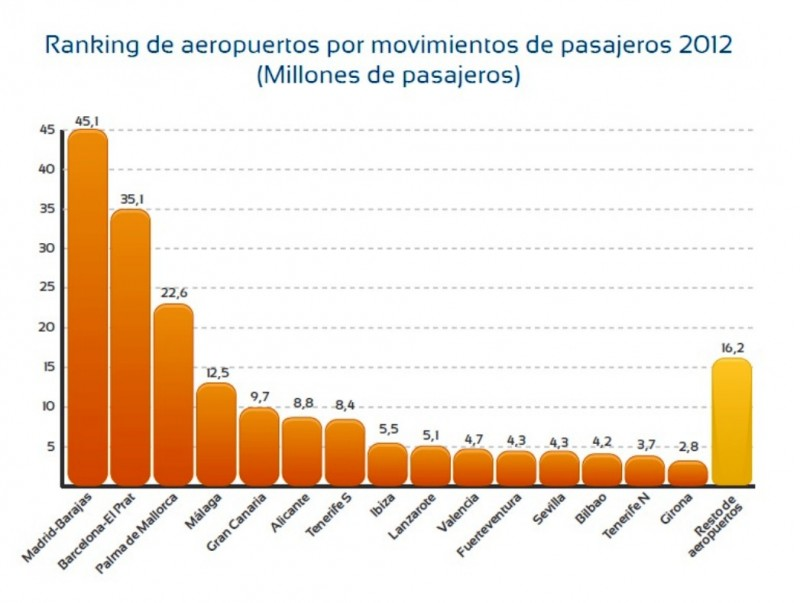
\includegraphics[width=0.7\textwidth]{./imagenes/introduccion/Ranking_de_aeropuertos_espayoles_por_pasajeros_horiz.jpg}
		\caption{Viajeros en aeropuertos españoles}
		\label{fig: Viajeros en aeropuertos españoles}
	\end{center}
\end{figure}	

Para tratar de solucionar este problema, se creó en 1988 el Central Flow management Unit, entidad dependiente de EUROCONTROL cuyo contenido es centralizar y estructurar todo el tráfico europeo, al igual que hace el Air Traffic Control System Command Center en Estados Unidos. Estas organizaciones trabajam para gestionar el tráfico aéreo a 3 niveles:
\begin{itemize}
	\item \textbf{Planificación táctica:} se realizan el mismo día, se encarga de manajar las situaciones en cada momento determinado
	\item \textbf{Planificación pre-táctica:} llevada a cabo con 2 días de antelación, se encarga de analizar el tráfico de los días previos, así como la previsión meteorológica.
	\item \textbf{Planificación estratégica: }se lleva a cabo 2 veces al año. En ella se se elaboran los planes de vuelo para cada compañía.
\end{itemize}


	
A pesar de todas las planificaciones, datos estadísticos, y mejoras en la previsión meteorológica, sigue existiendo un porcentaje importante de retrasos y cancelaciones. Según datos de EUROCONTROL, en el año 2016 un 20\% de los vuelos tuvieron un retraso mayor de 15 minutos
\begin{figure}[H]
	\begin{center}
		\centering
		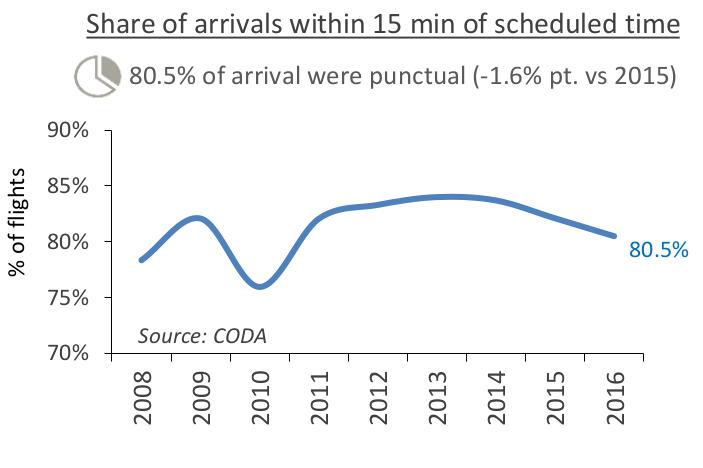
\includegraphics[width=0.7\textwidth]{./imagenes/introduccion/retrasos.png}
		\caption{Porcentaje retrasos en 2016}
		\label{fig: Porcentaje retrasos en 2016}
	\end{center}
\end{figure}

El tipo de retraso depende de la zona que estudiemos: en Estados Unidos la mayor parte de los retrasos se debe a un cuello de botella que existe en sus aeropuertos, mientras que en europa es la sobresaturación de espacios aéreos el principal problema, ya que hay un gran núnmero de aeropuertos con mucho tráfico muy cercanos unos de otros, mientras que en EEUU están más dispersos.
\begin{figure}[H]
	\begin{center}
		\centering
		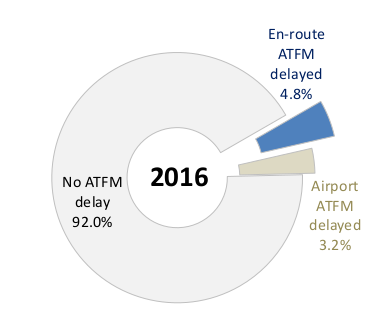
\includegraphics[width=0.7\textwidth]{./imagenes/introduccion/tiposRetrasos.png}
		\caption{Causas posibles de retraso de un vuelo}
		\label{fig: Causas posibles de retraso de un vuelo}
	\end{center}
\end{figure}

A lo largo de los últimos tiempos se han desarrollado varios modelos cuya finalidad es tratar de resolver (o l menos minimizar) el problema. Debido a que la causa más importante de los retrasos se debe al propio aeropuerto, la mayoría de los modelos se centran en tratar de resolver este cuello de botella. \\
Sin embargo, existen también modelos más complejos que también tienen en cuentya el espacio aéreo. Algunas de las estrategias que se aplican son:

\begin{enumerate}
	\item \textbf{Singe-Airport Ground-Holding Problem (SAGHP):} poco utilizada a excepción de algunos aeropuertos italianos, este modelo tiene en cuenta el número de despegues y aterrizajes que puede soportar un aeropuerto por unidad de tiempo.
	\item \textbf{Multi-Airport Ground-Holding Problem (MAGHP): }muy similar a la anterior, salvo que maneja varios aeropuertos de forma conjunta, teniendo en cuenta las relaciones entree ellos.
	\item \textbf{Air Traffic Flow Management Problem (ATFMP)}: introduce en el modelo el espacio aéreo. Como se puede ver en la figura \ref{fig: Causas posibles de retraso de un vuelo}, el porcentaje de retrasos en ruta fue mayor que el retraso en tierra. Esto se debe a que en los diferentes sectores aéreos las restricciones son menores que en los propios aeropuertos, por lo que un retraso en ruta no conlleva un retraso en otros vuelos, mientras que un retraso en un aeropuerto implica un retraso en el resto de vuelos que han de partir desde el mismo aeropuerto.
	\begin{figure}[H]
		\begin{center}
			\centering
			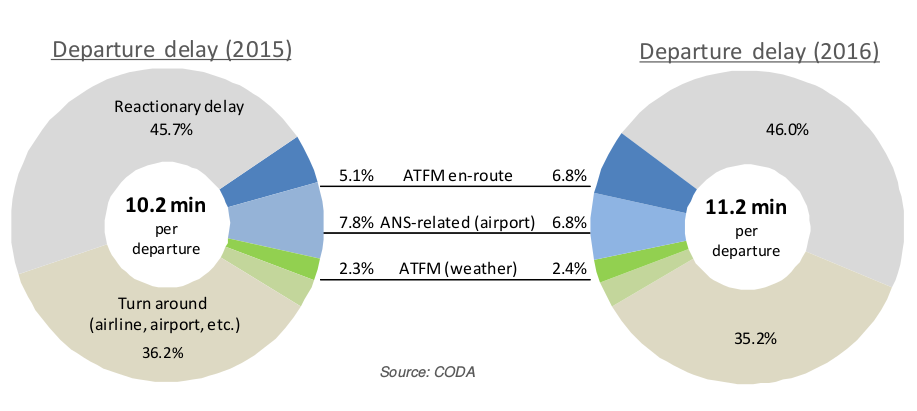
\includegraphics[width=0.7\textwidth]{./imagenes/introduccion/retrasosSalida.png}
			\caption{Comparativa retrasos 2015-2016}
			\label{fig: Comparativa retrasos 2015-2016}
		\end{center}
	\end{figure}
	\item \textbf{Air Traffic Flow Management Rerouting Problem (ATFMRP): }muy similar a ATFMP, pero añade además la posibilidad de desviar vuelos.
	\begin{figure}[H]
		\begin{center}
			\centering
			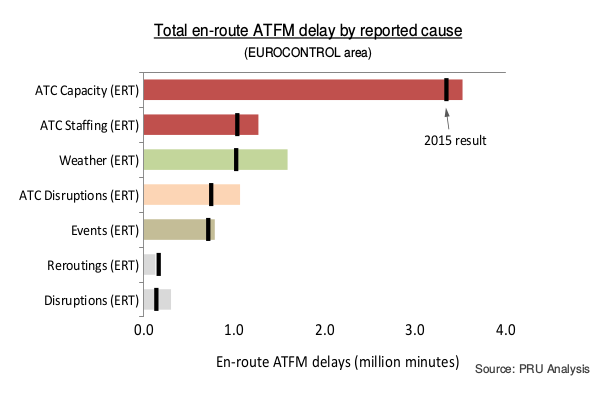
\includegraphics[width=0.7\textwidth]{./imagenes/introduccion/rerouting.png}
			\caption{Retrasos en 2016}
			\label{fig: Retrasos en 2016}
		\end{center}
	\end{figure}
	\item \textbf{Air Traffic Flow Management Rerouting with Flight Cancellation Problem (ATFMRCP): }añade la posibilidad de cancelar vuelos. Se trata de un modelo más teórico que práctico, ya que la opción de cancelar vuelos no es una opción válida para casos reales.
\end{enumerate}

\section{Versiones anteriores}
Este Trabajo Final de Grado es la continuación del trabajo que llevaron a cabo Diego Ruiz Aguado y Gonzalo Quevedo García en 2012 en sus Proyectos Finales de Carrera, los cuales se apoyaron a su vez en la Tesis Doctoral de Alba Agustín  Martín (2011).\\

A continuación se hace una breve descripción del trabajo de  Diego Ruiz Aguado y Gonzalo Quevedo García:
\begin{enumerate}
	\item Los datos del problema se encontraban en una base de datos no relacional con redundancias. El primer paso consistió en migrar esta base de datos no relacional a una base de datos MySQL relacional y bien estructurada.
	\item Para obtener los datos que necesitaba el problema, se realizó un programa en JAVA que se conectaba a la BBDD y creaba varios ficheros .txt en la que se volcaba toda la información necesaria para el posterior modelado del problema.
	\item A continuación, el programa en java leía estos ficheros .txt y creaba las estructuras de datos necesarias(árbol de rutas, vuelos, wapoints, etc).
	\item Posteriormente una subrutina en C se encargaba de definir un problema de CIPLEX con la función objetivo y las restricciones necesarias.
	\item Finalmente, se ejecutaba el problema de optimización mediante la librería CIPLEX para obtener la mejor solución del problema.
\end{enumerate}

Debido al enfoque teórico de este Trabajo de Fin de Grado, el modelo que se va a implementar se basa en el ATFMRCP, ya que permitirá cancelaciones, retrasos en aeropuertos, retrasos en ruta y desvíos. 

\section{Nuevos objetivos}
La versión anterior del problema adolecía de un importante inconveniente: no podía salir de los máximos locales, ya que el heurístico que se utilizaba para lanzar los vuelos era un algoritmo voraz. De esta forma, el resultado del problema dependía en gran medida del orden en que se intentara encontrar una solución para cada vuelo.\\

Por tanto los objetivos marcados para este Trabajo de Fin de Grado han sido los siguientes (ordenados en decreciente prioridad):
\begin{enumerate}
	\item \textbf{Mejorar heurístico: }el objetivo principal de este TFG consiste en sustituir el algoritmo voraz por un heurístico que permita al problema escapar de los máximos locales, y por tanto encontraqr una solución mejor al problema.
	\item \textbf{Desacoplar el programa de CIPLEX: }con la implementación de los nuevos heurísticos no es necesaria la librería de optimización. Se pasará de un sistema clásico de optimización (función objetivo y restricciones) a una estructura de objetos que permitan un manejo óptimo de las estructuras de datos durante la ejecución del algoritmo.
	\item \textbf{Mejorar el sistema de lectura de datos: }la versión actual del programa crea ficheros .txt en los que se vuelca toda la A2 del problema (vuelos, waypoints, routas, etc) que pueden superar las 100.000 lineas. Estos ficheros auxiliares pueden sustituirse por ficheros mucho más pequeños en los que se exporta la A2 de la base de datos, y de forma interna el problema se encarga de crear las estructuras necesarias.
	\item \textbf{Representación gráfica: }aunque estrictamente no aporta a mejorar la solución del problema, su representación gráfica puede ayudar a modelizar mejor el algoritmo, ya que permite visualizar de manera rápida y sencilla el estado del problema .
\end{enumerate}
	\chapter{Descripción del problema}
\label{descripción}
El modelo implementado se puede resumir como un espacio aéreo dividido en diferentes sectores por el que viajan una serie de aviones. Los vuelos parten y finalizan de un aeropuerto, y tienen una serie de rutas para llegar a su destino.

El objetivo del problema es encontrar una solución factible al mayor número de vuelos cumpliendo una serie de restricciones. Las entidades de las que se compone el modelo son sectores, waypoints, vuelos, rutas y waypointsRoute. A continuación se describe con más detalle las características de cada uno de estos elementos.


\section{Sectores}
Representan las diferentes zonas en las que se divide el espacio aéreo. Los sectores tienen un límite de capacidad, de modo que para un instante e tiempo $t$ solo puede haber un número $n$ de vuelos simultáneamente en un sector. De este modo, si un vuelo tiene programada una ruta en un momento de tiempo que pasa por un sector que está al límite de su capacidad, esa ruta no será válida, por lo que tendrá que intentar retrasar su ruta, usar una ruta alternativa, y si no tiene otra opción, cancelarse.

Para las pruebas que hemos realizado se ha considerado el escenario más restrictivo posible: la capacidad de un sector en cada instante de tiempo es 1.

\section{Waypoints}
Los waypoints representan puntos de ruta en las trayectorias de los vuelos a través del espacio aéreo. Dependiendo de su ubicación, los waypoints pueden estar en el interior del sector, por ejemplo en el caso de los aeropuertos, o en la intersección entre dos o más sectores para representar el paso de un sector a otro.


\begin{figure}[h]
	\begin{center}
		\centering
		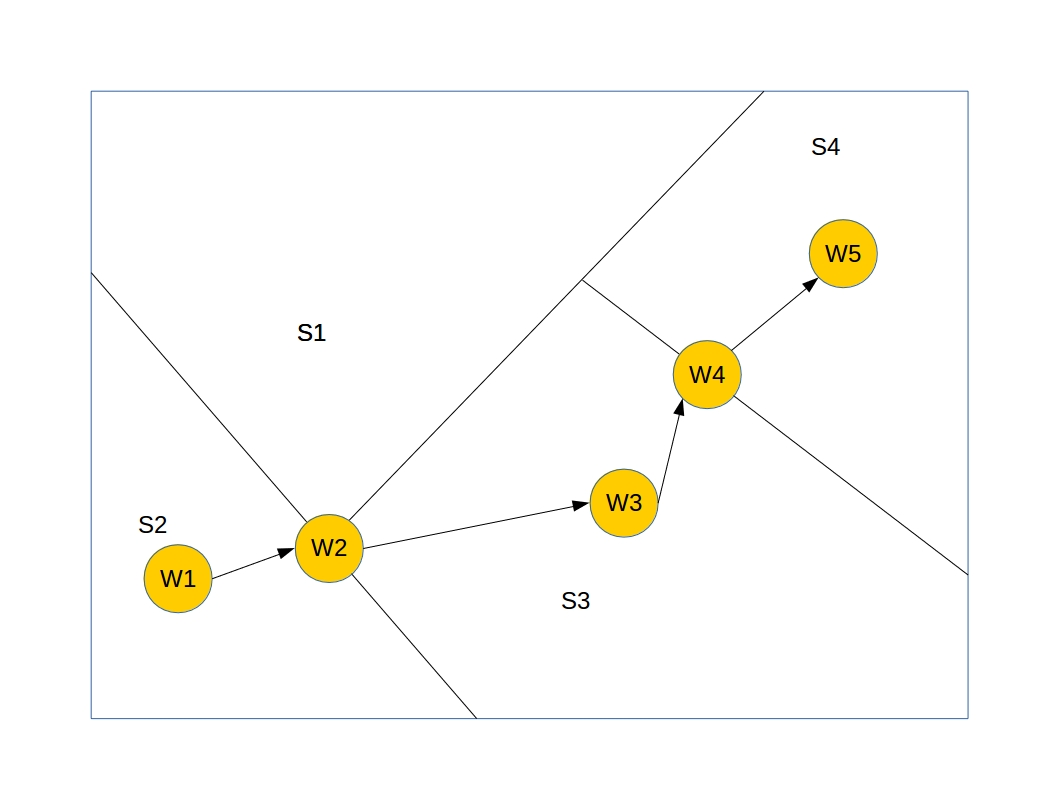
\includegraphics[width=0.9\textwidth]{./imagenes/descripcion_problema/sectoresYWaypoints.jpg}
		\caption{Ejemplo sectores y waypoints.}
		\label{fig: Ejemplo sectores y waypoints}
	\end{center}
\end{figure}


\section{Vuelos}
Los vuelos parten siempre de un Waypoint aeropuerto y a través de una serie de rutas preasignadas, que marcan los posibles itinerarios de vuelo a través de Waypoints, llegan a un aeropuerto destino. Los vuelos pueden llegar a su aeropuerto de destino por cualquiera de sus rutas, así como también retrasar su itinerario si fuera necesario, pero si debido a las restricciones del problema no se encontrara una solución factible, el vuelo sería cancelado.

Por tanto, los vuelos se pueden clasificar en función de su estado al final del problema en:
\begin{itemize}
	\item \textbf{Vuelos programados:} se ha encontrado una ruta para el vuelo que cumple con las restricciones del problema. A su vez, los vuelos con solución se pueden subdividir en
	\begin{itemize}
		\item \textbf{Solución por defecto:} la solución del vuelo es la ruta inicial sin retrasos. Es el mejor resultado posible.
		\item \textbf{Retrasado:} se encuentra una solución factible en la ruta por defecto del vuelo, pero se ha producido un retraso entre alguno de sus waypoints.
		\item \textbf{Desviado:} la solución encontrada para el vuelo no es la ruta a priori. Puede ser tan corta como la solución por defecto.
	\end{itemize}
	\item \textbf{Vuelos no programados} no se ha podido localizar ninguna ruta factible para el vuelo, por lo que se considera como cancelado.
\end{itemize}
Los vuelos tienen un coste de cancelación y están asociados a determinadas aerolíneas.

\section{Rutas}
Las rutas son el conjunto de trayectorias que tiene un vuelo para llegar desde su aeropuerto de origen al de destino, y se representan como un grafo ponderado y dirigido en el que el coste de cada arista coincide con el intervalo de valores entre los cuales un vuelo puede hacer el trayecto entre 2 waypoints.

De todas las posibles rutas, una es la que se toma como ruta preestablecida, y es la que se indica en el plan de vuelo original. Esta ruta predefinida será siempre igual o mejor (más rápida) que el resto de sus rutas. El objetivo del problema es encontrar un plan de vuelo que suponga la menor variación posible sobre el plan de vuelo original.

Una de las características más importantes del modelo es que se permite que un vuelo pueda retrasar su trayecto entre 2 waypoints, normalmente para no coincidir en el tiempo y el espacio con otro vuelo o porque el sector al que intenta acceder está sobrecargado.\\

Por tanto en cada trayectoria entre waypoints se permite un retraso máximo, de forma que entre 2 waypoints un vuelo puede recorrer esa distancia entre
\begin{equation}
[T_{mín} , T_{máx}]
\end{equation}

\noindent, donde $T_{mín}$ y $T_{máx}$ son el tiempo mínimo y máximo en el que un vuelo puede ir desde un waypoint a otro, respectivamente.\\

Para modelar que los aeropuertos no tienen capacidad, creamos unos waypoints $aeropuerto'$ que simulan el waypoint en el que los vuelos aterrizan o despegan (estos waypoints sí que tienen las restricciones habituales del resto de waypoints). Por ejemplo, un vuelo entre 2 aeropuertos con un waypoint entre ellos en el que se permita en cada trayectoria un retraso de 1, daría como resultado el siguiente grafo:
\begin{figure}[h]
	\centering
	\documentclass{standalone}
\usepackage{tikz}
\begin{document}
\begin{tikzpicture}[->,>=stealth',shorten >=1pt,auto,node distance=3cm,
thick,main node/.style={circle,draw,font=\sffamily\Large\bfseries}]

\node[main node] (1) {$A1$};
\node[main node] (2) [right of=1] {$A1'$};
\node[main node] (3) [right of=2] {$W1$};
\node[main node] (4) [right of=3] {$A3'$};
\node[main node] (5) [right of=4] {$A3$};


\path[every node/.style={font=\sffamily\small}]
(1) edge node {$\{0,1\}$} (2)
(2) edge node {$\{1,2\}$} (3)
(3) edge node {$\{1,2\}$} (4)
(4) edge node {$0$} (5);
\end{tikzpicture}
\end{document}
	\caption{Ejemplo ruta de un vuelo.}
	\label{fig: Ejemplo ruta de un vuelo}
\end{figure}

En este ejemplo, el retraso entre $A1$ y $A1'$ representa el retraso en tierra que se permite para el vuelo. El retraso entre los nodos $A3'$ y $A3$, al igual que en cualquier conexión entre los nodos $aeropuerto\_aterrizaje'$ y $aeropuerto\_aterrizaje$ será siempre 0, ya que no tiene sentido que un vuelo que llega a su aeropuerto de destino retrase su ruta.


\section{Waypoint Route}
Los waypoint route son la entidad que representa los waypoints en diferentes instantes de tiempo. Los waypoint routes son necesarios para crear el grafo de recorridos \textit{completo} de un vuelo, ya que si en alguno de sus trayectos un vuelo permite algún retraso, obtendremos que las aristas del grafo representan a un conjunto de valores. Dado que los waypoint route dependen de las rutas de cada vuelo, los waypoints route son únicos para vuelo, de forma que el grafo de recorrido de cada vuelo es independiente de los otros vuelos.\\

Para crear el grafo que represente las posibles rutas de un vuelo y todos sus posibles retrasos, tenemos que crear un nodo por cada waypoint en cada posible instante de tiempo $t$. De esta forma, tendremos un grafo con un conjunto de nodos de la forma $W_{t}$, siendo $W$ el nombre del waypoint y $t$ el instante de tiempo.\\
Tras realizar este proceso, se incorpora al modelo que un vuelo puede estar en el mismo waypoint en diferentes momentos de tiempo si se ha elegido otra ruta más larga o se ha producido un retraso.\\

En el ejemplo de \autoref{fig: Ejemplo ruta de un vuelo}, la forma expandida del grafo sería (suponiendo que el vuelo despega en el instante $t=0$) correspondería con la \autoref{fig: Ejemplo grafo de recorridos de un vuelo}:
\begin{figure}[h]
	\centering
	\scalebox{.6}{\documentclass{standalone}
\usepackage{tikz}
%\usetikzlibrary{...}
\begin{document}
	\begin{tikzpicture}[->,>=stealth',shorten >=1pt,auto,node distance=3cm,
	thick,main node/.style={circle,draw,font=\sffamily\Large\bfseries}]
	
	\node[main node] (1) {A1};
	\node[main node] (2) [above right of=1] {$A1'_{0}$};
	\node[main node] (3) [below right of=1] {$A1'_{1}$};
	\node[main node] (4) [above right of=2] {$W1_{2}$};
	\node[main node] (5) [below right of=2] {$W1_{3}$};	
	\node[main node] (6) [above right of=4] {$A3'_{4}$};
	\node[main node] (7) [below right of=4] {$A3'_{5}$};		
	\node[main node] (8) [below right of=5] {$A3'_{6}$};		
	\node[main node] (9) [below right of=3] {$W1_{4}$};		
	\node[main node] (10) [below right of=9] {$A3'_{7}$};		
	\node[main node] (11) [below right of=7] {A3};		
	
	\path[every node/.style={font=\sffamily\small}]
	(1) edge node {0} (2)
	edge node {1} (3)
	(2) edge node {2} (4)	
	edge node {3} (5)
	(3) edge node {2} (5)
	edge node {3} (9)	
	(4) edge node {2} (6)	
	edge node {3} (7)
	(5) edge node {2} (7)
	edge node {2} (8)
	(9) edge node {2} (8)
	edge node {3} (10)
	(6) edge node {0} (11)
	(7) edge node {0} (11)
	(8) edge node {0} (11)
	(10) edge node {0} (11);	
	\end{tikzpicture}
\end{document}



}
	\caption{Ejemplo grafo de recorridos de un vuelo.}
	\label{fig: Ejemplo grafo de recorridos de un vuelo}
\end{figure}


Un vuelo puede además tener más de una ruta. En este caso el grafo de recorridos tendrá más de un camino para llegar al nodo de destino:
\begin{figure}[h]
	\centering
	

\documentclass{standalone}
\usepackage{tikz}
%\usetikzlibrary{...}
\begin{document}
		\begin{tikzpicture}[->,>=stealth',shorten >=1pt,auto,node distance=3cm,
		thick,main node/.style={circle,draw,font=\sffamily\Large\bfseries}]
		
		\node[main node] (1) {$A1$};
		\node[main node] (2) [right of=1] {$W1$};
		\node[main node] (3) [right of=2] {$A3$};
		\node[main node] (4) [below of=2] {$W2$};

		
		\path[every node/.style={font=\sffamily\small}]
		(1) edge node {$\{2,3\}$} (2)
		(2) edge node {$\{1,2\}$} (3)
		(1) edge node {$\{3,5\}$} (4)
		(4) edge node {$\{1,2\}$} (3);
		
		\end{tikzpicture}
\end{document}
	\caption{Ejemplo vuelo con 2 rutas.}
	\label{fig: Ejemplo vuelo con 2 rutas}
\end{figure}

Su grafo de recorridos se compondría de forma análoga a los anteriores como se puede ver en la \autoref{fig: Ejemplo grafo recorridos con 2 rutas}
\begin{figure}[]
	\centering
		\scalebox{1}{\documentclass{standalone}
\usepackage{tikz}
%\usetikzlibrary{...}
\begin{document}
	\begin{tikzpicture}[->,>=stealth',shorten >=2pt,auto,node distance=4cm,
	thick,main node/.style={circle,draw,font=\sffamily\Large\bfseries}]
	
	\node[main node] (1) {A1};
	\node[main node] (2) [above right of=1] {$A1'_{0}$};
	\node[main node] (3) [below right of=1] {$A1'_{1}$};
	\node[main node] (4) [above right of=2] {$W1_{2}$};
	\node[main node] (5) [below right of=2] {$W1_{3}$};	
	\node[main node] (6) [above of=7] {$A3'_{4}$};
	\node[main node] (7) [above left of=11] {$A3'_{5}$};		
	\node[main node] (8) [below left of=11] {$A3'_{6}$};		
	\node[main node] (9) [below left of=10] {$W1_{4}$};		
	\node[main node] (10) [below of=8] {$A3'_{7}$};		
	\node[main node] (11) [below right of=7] {A3};		
	\node[main node] (12) [above left of=6] {$W2_{3}$};		
	\node[main node] (13) [below left of=8] {$W2_{4}$};	

	\path[every node/.style={font=\sffamily\small}]
	(1) edge node {0} (2)
	edge node {1} (3)
	(2) edge [blue] node {2} (4)	
	edge [blue] node {3} (5)
	edge [red] node {3} (12)
	edge [red] node {4} (13)
	(3) edge [blue] node {2} (5)
	edge [blue] node {3} (9)	
	edge [red] node {3} (13)

	(4) edge [blue] node {2} (6)	
	edge [blue] node {3} (7)
	(5) edge [blue] node {2} (7)
	edge [blue] node {2} (8)
	(9) edge [blue] node {2} (8)
	edge [blue] node {3} (10)
	(6) edge node {0} (11)
	(7) edge node {0} (11)
	(8) edge node {0} (11)
	(10) edge node {0} (11)
	(12) edge [red] node {1} (6)
	(13) edge [red] node {1} (7)
		;	
	\end{tikzpicture}
\end{document}



}
	\caption{Ejemplo grafo recorridos con 2 rutas: ruta 1 en \textcolor{blue}{azul} y ruta 2 en \textcolor{red}{rojo}.  }
	\label{fig: Ejemplo grafo recorridos con 2 rutas}
\end{figure}



\section{Descripción del modelo}
Por tanto, el problema se puede resolver mediante un modelos de optimización combinatoria lineal con los siguientes elementos:
\begin{itemize}
	\item \textbf{Función objetivo: }hay que maximizar el número de vuelos a los que se les encuentra una solución factible.\\
	 Dado que los vuelos no tienen solución binaria (cancelado/con solución), sino que dentro de las soluciones factibles hay unas mejores que otras, se ha creado un sistema de evaluación de vuelos con solución factible: los vuelos colocados en su solución a priori aportan 5 pts, los retrasados 3, los desviados en tiempo 2 y los desviados y retrasados 1.\\
	 Este sencillo sistema se ideó para evaluar lo factible que es una solución, ya que como se explicó anteriormente no estamos utilizando el coste de cancelación (en ese caso se trataría de un problema de minimización de costes, en vez de maximizar la solución).
	\item \textbf{Restricciones:} el modelo tiene tan sólo dos:
	\begin{enumerate}
		\item Para cualquier instante de tiempo $t$, no puede haber más de 1 vuelo en un arco que conecta 2 waypoints. 
		\item Dado cualquier instante de tiempo $t$, no puede haber más de $n$ vuelos simultáneamente en el mismo sector. Aunque $n$ es un parámetro variable, todas las pruebas que hemos realizado hemos usado $n=1$, poniéndonos así en el caso más estricto de todos.
	\end{enumerate}
\end{itemize}

\section{Modelo base de datos}
Como ya se ha explicado, no se ha realizado ninguna modificación sobre la base de datos obtenida en la versión anterior del problema de 2012. El diagrama de entidad relación es el siguiente:
\begin{figure}[H]
	\begin{center}
		\centering
		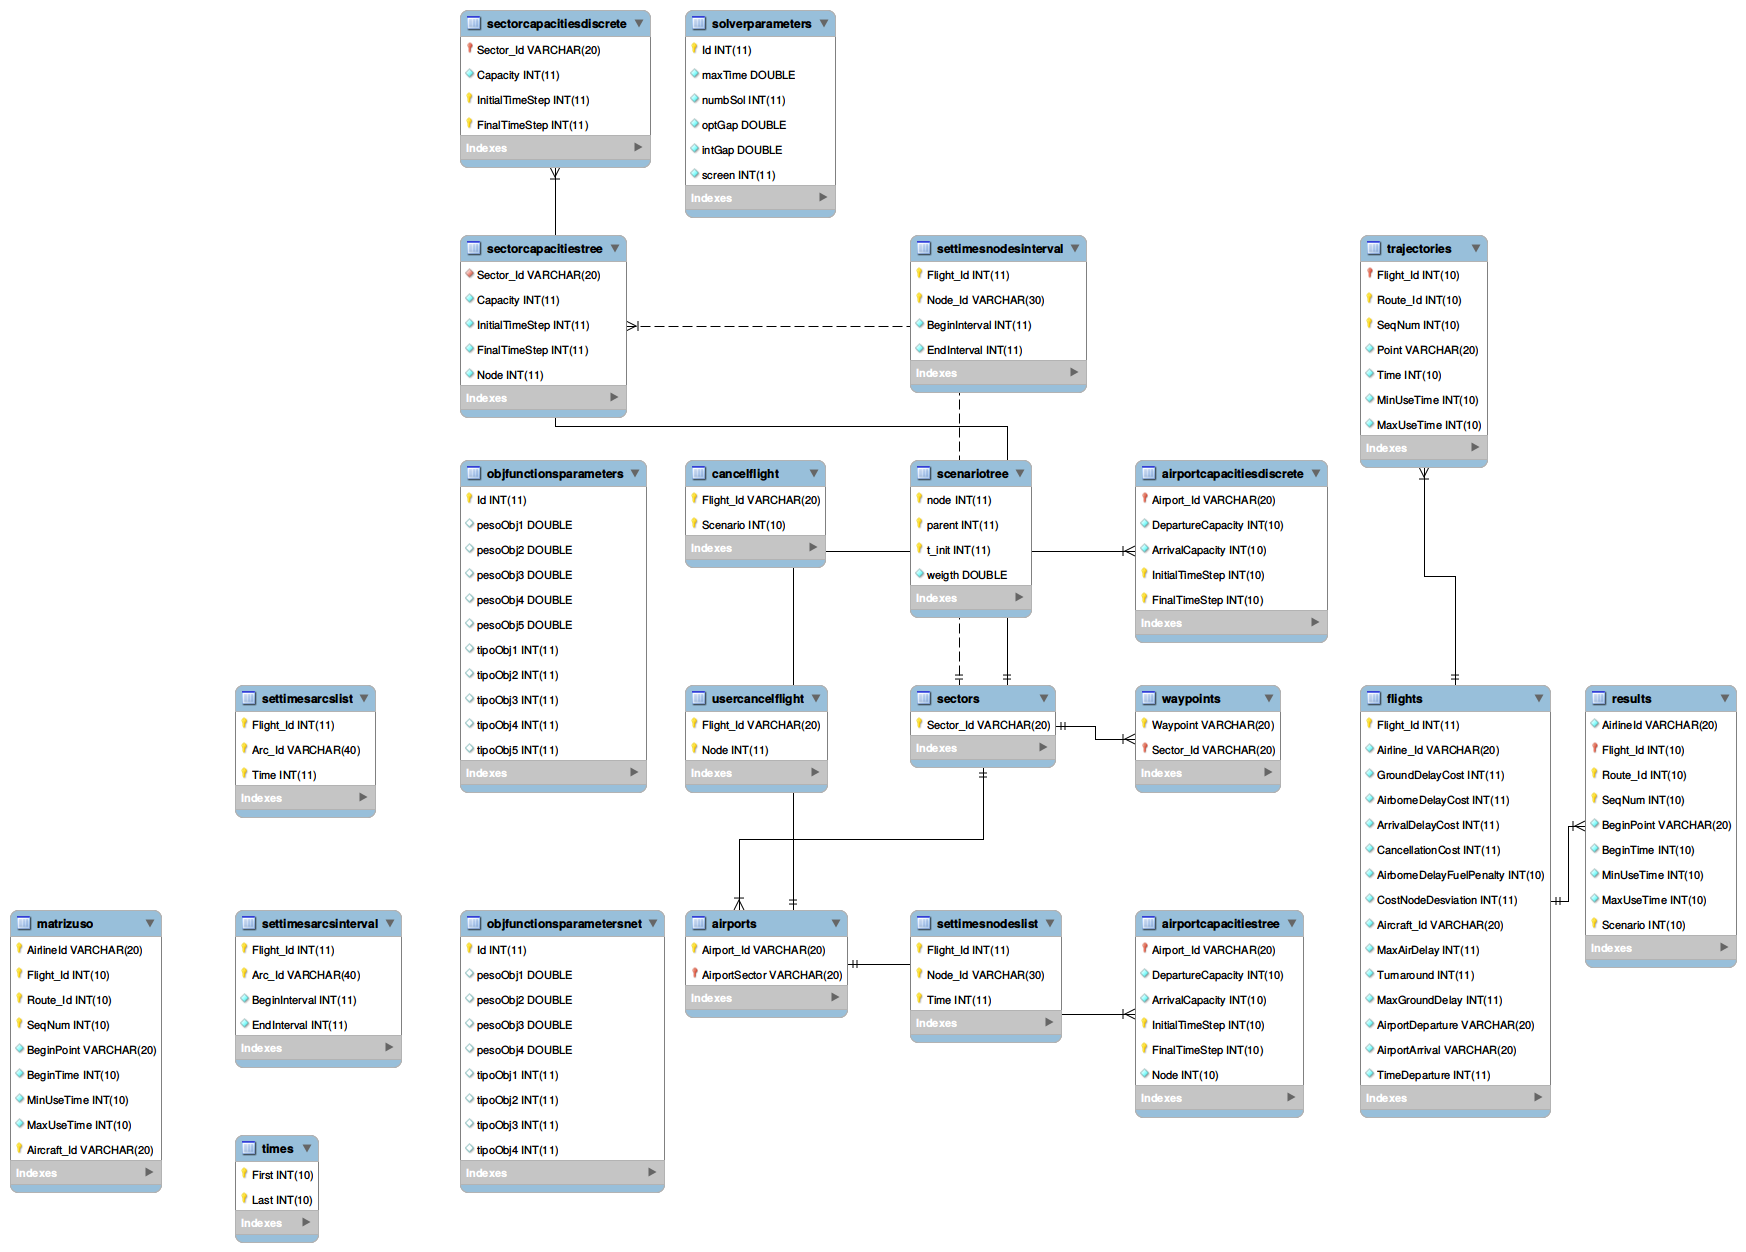
\includegraphics[width=1\textwidth]{./imagenes/descripcion_problema/bbdd.png}
		\caption{Modelo BBDD.}
		\label{fig: Modelo BBDD}
	\end{center}
\end{figure}

	\chapter{Tecnologías utilizadas}
\label{tecnologías}
Las tecnologías que se han utilizado a lo largo de este Trabajo de Fin de Grado han sido las siguientes:

\section{C++}
Todo el código ha sido desarrollado utilizando el lenguaje C++, creado por  Bjarne Stroustrup en 1983. C++ sigue el paradigma de programación imperativa, y es considerado un lenjuaje orientado a objeto híbrido al ser una extensión del lenguaje C. Desde los años 90 se ha mantenido como uno de los lenguajes más utilizados, y actualmente ocupa el puesto 3º en el rankin \href{http://www.tiobe.com/tiobe-index/}{TIOBE}.\\

Aunque se comenzó utilizando C en las primeras versiones del TFG, finalmente se optó por utilizar C++. Esto fue debido principalmente a 4 factores, que son además las ventajas de C++ sobre C:
\begin{itemize}
	\item \textbf{Permite la orientación a objetos: }a la hora de modelar de nuevo el problema, era necesario crear una estructura de objetos que permitieran un fácil manejo de los datos, y características de la orientación a objetos como la herencia o los constructores permitía manejar la información de forma sencilla y estructurada.
	\item \textbf{Estructuras de datos: }aunque en C también existen, en C++ ya vienen implementadas como parte básica del lenguaje. El uso de estructuras como vectores, tuplas o mapas (y sus métodos) permiten implementaciones más sencillas y eficientes, que reducen en gran medida el tiempo de programación.
	\item \textbf{Sigue permitiendo un manejo de memoria a bajo nivel: }debido a la índole del problema este punto era muy importante, ya que un mal uso de la memoria podría hacer inviables problemas demasiado grandes o con muchas iteraciones.
	\item \textbf{Portabilidad:} el cambio de C a C++ es prácticamente inmediato, por lo que se pudo reaprovechar todo el trabajo realizado.
\end{itemize}
                  

\section{MySQL}
MySQL es un sistema relacional de gestión de base de datos multiplataforma desarrollado en ANSI C y C++ en 1995 por Michael Widenius. Actualmente es uno de los 3 sistemas de BBDD más utilizados del mundo, junto a Oracle y Microsoft SQL Server.

A pesar de ser un proyecto de Apache, está patrocinado por la empresa Oracle que posee la mayororía de los derechos, lo que ocasionó que en 2009 varios antiguos desarroladores de MySQL crearan MariaDB, un fork\footnote{Un fork es la creación de un proyecto software con un nuevo propósito a partir de código ya existente.} de MySQL con licencia opensource.\\

Al igual que en la versión anterior del proyecto, la BBDD que usamos será la relacional que realizó Diego Ruiz Aguado en el 2012. En esta base de datos se encuentran todos los datos del problema: waypoints, rutas, aeropuertos, vuelos ... etc, los cuales serán utilizados para crear la estructura del problema.


\section{HTML y JavaScript}
\textbf{HTML} (HyperText Markup Language) es un lenguaje de marcado creado por Tim Berners-Lee en 1991 para la creación de páginas web. Es el lenguaje más utilizado para la elaboración de páginas web, además de un estándar a cargo del consorcio WWW.
HTML se considera el lenguaje web más importante (entre todos los lenguajes alternativos a HTML no alcanzan el 0.001\% de uso ) y ha tenido un impacto muy importante en la expansión del WWW. Entre sus funcionalidades básicas de HTML 5 (la última versión liberada) se encuentran funcionionalidades como añadir audio, vídeo, canvas o \textit{drag and drop}.

\textbf{JavaScript} es un lenguaje de programación interpretado, imperativo, dinámico, débilmente tipado y  orientado a objetos. Es parte del estándar ECMAScript, soportado por la gran mayoría de los navegadores desde 2012, lo que lo convierte en el lenguaje más utilizado para el lado cliente en aplicaciones web. 
JS se basa en el manejo del DOM (Document Object Model) de código HTML y algunas de sus funcionalidades más sencillas podrían ser el de crear contenido interactivo, animaciones o validacuión de formularios. Sin embargo, debido a la popularidad de los últimos años, las funcionalidades de JS, y principalmente, de frameworks para aplicaciones web \footnote{Un framework para aplicaciones web es un conjunto de tecnologías, módulos de desarrollo, y capas de abstracción destinadas a facilitar el desarrollo.} han hecho que el lenguaje incorporar un gran número de mejoras como peticiones asíncronas, funciones lambda, funciones de orientación a objetos,... etc.
Actualmente el ritmo al que se crean nuevas tecnologías basadas en JavaScript es elevadísimo, habiendo multitud de frameworks como \href{https://angularjs.org/}{AngularJS} (desarrollado por Google), \href{https://facebook.github.io/react/}{ReactJS} (desarrolado por Facebook),\href{https://www.emberjs.com/}{EmberJS}, lenguajes derivados como \href{https://www.typescriptlang.org/}{TypeScript} que permiten añadir funcionalidades de tipado, o gran cantidad de librerías como \href{https://d3js.org/}{Data-Driven Documents}.\\

Para la representación gráfica del problema se ha utilizado JS para leer y parsear la información almacenada en un fichero y HTML para su visualización (para la creación del grafo se ha utilizado la librería \href{http://visjs.org/docs/network/}{vis.js}).

\section{Git y Github}
Git es un software de control de versiones distribuido creado por Linus Torvalds en 2005, cuyos dos mayores sistemas de hosting son Bitbucket y Github. Un sistema de control de versiones permite gestionar los cambios llevados a cabo sobre documentos a lo largo del tiempo, así como coordinar el trabajo de diferentes desarrolladores trabajando sobre el mismo documento simultáneamente.

La importancia de Github en los últimos años ha ido en aumento al haberse convertido en el repositorio de proyectos openSource  muy importantes como el framework \href{https://github.com/twbs/bootstrap}{Bootstrap}, el lenguaje de lado de servidor \href{https://github.com/nodejs/node}{Node.js}, la librería \href{https://github.com/jquery/jquery}{Jquery} o el framework del lenguaje Ruby \href{https://github.com/jquery/jquery}{Rails}.\\

Se ha utilizado Git como sistema de versiones debido a las facilidades que otorga para trabajar desde distintos terminales, así como su fácil manejo de versiones . Todo el código se puede descargar y consultar en  \href{https://github.com/cavasanchez/TFG}{Github}.


	\chapter{Heurístico}
El algoritmo heurístico que se ha creado para el problema está inspirado en el metahurístico \textit{GRASP (Greedy Randomized Adaptive Search Procedure)}, sobre el que se han realizado una serie de modificaciones para adaptarlo al modelo en cuestión. A continuación se explicará el funcionamiento de un GRASP, para después explicar el algoritmo propuesto comparando sus diferencias y semajanzas.

\section{GRASP}
Un Grasp es un metaheurístico constructivo desarrollado inicialmente por T. Feo   M. Resende, y se definie como \textcolor{red}{->cita libro Abraham<-} \textit{un GRASP es un procedimiento multiarranque en el que cada arranque se corresponde con una iteración. Cada iteracción tiene dos fases bien diferenciadas, la fase de construcción, que se encarga de obtener una solución factible de alta calidad; la fase de mejora, que se basa en la optimización (local) de la solución obtenida en la primera fase.}

\subsection{Fase constructiva}
La fase constructiva es un proceso iterativo en el que se construye una solución elemento a elemento.\\
Inicialmente se parte de un componente o conjunto de componentes que conforman una solución parcial, y no serán seleccionables. Posteriormente se ordenan los elementos seleccionables utilizando una función voraz (Greedy), la cual asignará a cada elemento un valor que indique como variaría la función objetivo si se añade a la solución parcial.\\
Una vez están ordenados todos los elementos seleccionables, hay que seleccionar qué elemento es añadido a la solución parcial. GRASP no añade el mejor candidato posible, ya que esto no garantiza que se obtenga la solución óptima, sino que se elije aleatoriamente un candidato del conjunto de candidatos restringido (o RCL por sus siglas en inglés). Para crear esta RCl, se crea un conjunto de candidatos que cumplan
\begin{equation}\\
{RCL}_{umbral} = (c_{min}+\alpha(c_{max} - c_{min} ))
\end{equation}
donde $c_{min}$ y $c_{max}$ son respectivamente los valores más bajo y más alto del coste asignado a los elementos seleccionables, y el parámetro  :$\alpha : 0\leq \alpha \leq1$ determina el umbral permitido, de forma que se escoge un candidato aleatorio. Si fijamos $\alpha=1$, en la RCL solo contaríamos con el mejor candidato, y sería una función miope pura. Por el contrario si fijamos $\alpha=0$, serán seleccionados todos los candidatos.\\

Una vez seleccionado el elemento o elementos, se introducen en la solución parcial y se les marca como no seleccionables. El resto de candidatos siguen siendo seleccionables, por tanto cuando se les vuelva a evaluar para ser candidatos, sus valores serán distintos a los de la iteración anterior, ya que la solución parcial ha variado al haber añadido el último elemento conjunto de candidatos.\\

La fase constructiva finaliza cuando se dispone de una solución factible.
\subsection{Fase de mejora}
Pero la fase constructiva no garantiza que la solución sea óptima respecto a su vecindad. Por ello GRASP incorpora la fase de mejora, que consiste en un procedimiento de optimización local, el cual puede ser otra metaheurística o una función de búsqueda local.
\section{Heurístico implementado}
\subsection{Introducción}
El algoritmo diseñado para este problema se resume en el siguiente pseducódigo:\\

\begin{algorithm}[H]

	inizializarProblema()\;
	\While{$N < iteracionesMáximas$}{
		añadirVuelosEnColaCandidatos()\;
		lanzarVuelosSoloSoluionesIniciales()\;
		intercambiarVuelos()\;
		lanzarVuelosPermitiendoRetrasos()\;
		lanzarVuelosPermitiendoDesvíos()\;
		buscarWaypointsSinUsar()\;
		retrasarVuelos()\;
		\If{$N\%númeroSolucionesExaminar== 0$}{
			crearColaCandidatos()\;
		}
}
\caption{Esquema algoritmo implementado}
\end{algorithm}

Como se comentó anteriormente, al igual que un algoritmo GRASP tradicional, se compone de una fase constructiva en la que se obtiene una solución de alta calidad y una fase constructiva que se produce cada $N$ iteraciones, en la cual se analizarán las solucions anteriores para seleccionar los vuelos más prometedores y añadirlos al problema, de forma que tengan más posibilidad de ser seleccionados antes. A continuación se explican con más detalle ambas fases.



\subsection{Fase constructiva}
Dado que este problema tiene siempre una solución factible (cancelar todos los vuelos), el objetivo de esta fase es conseguir una solución de alta calidad. 

A continuación se detalla cada función que se lleva a cabo en la fase constructiva;:
\begin{enumerate}
	
	\item \textbf{Añadir vuelos a la cola de candidatos:} es el primer paso de la fase constructiva, y solo se lleva a cabo si en la iteración anterior se ha creado una cola de candidatos. Esta función se encarga de generar de forma aleatoria el orden en el que se lanzarán los vuelos en el siguiente paso del algoritmo. Funciona de la siguiente manera:
	\begin{enumerate}
		\item Si no hay cola de candidatos, se obtiene el id de cada vuelo del problema y se ordenan de forma aleatoria:
		\begin{multline}\\
			\{1,2,3,4,5\} \Rightarrow \{2,4,5,1,3\}\\
		\end{multline}
		\item Si por el contrario si que tenemos una cola de candidatos, juntaremos el array de ids de los vuelos del problema junto a el array de candidatos. posteriormente se ordenan y se descartan los elementos repetidos, de forma que los elementos que estén repetidos tendrán más posibilidades de estar al principio del array:
		\begin{multline}\\
		\{1,2,3,4,5\} + \{2,4\} = \{1,2,3,4,5,2,4\} \\
		\{1,2,3,4,5,2,4\} \Rightarrow \{2,5,4,3,1\}  \\ 
		\end{multline}
	\end{enumerate}
	
	\item \textbf{Lanzar vuelos con las soluciones iniciales: }se lanzan todos los vuelos de manera aleatoria sin permitir retrasos o desvíos, la única ruta que se permite es la solución por defecto.\\
	Tras realizar varias pruebas, se ha podido comprobar que los pasos siguientes del algoritmo dependen en gran medida de los vuelos a los que se encuentra solución en esta fase. Esto se debe a que un ``mal'' vuelo colocado en su solución inicial puede sobrecargar sectores clave para otros muchos vuelos. En las pruebas que hemos realizado, en esta fase se colocan con éxito entre un 5\% y un 15\% de los vuelos.
	
	\item \textbf{Intercambio de vuelos: } se intenta sustituir uno de los vuelos exitosos del paso anterior por 2 o más vuelos aleatorios a los que no se les halló solución.\\
	Este paso fue introducido para paliar el problema que se indicaba en el paso anterior, y se realiza partiendo de una idea básica: si cancelando un vuelo que teníamos con solución conseguimos colocar con éxito 2 o más vuelos, será siempre una mejora.\\
	
	Por ejemplo, si en la fase anterior fue colocado con éxito un vuelo de la siguiente forma
	\begin{figure}[H]
		\centering
		\documentclass{standalone}
\usepackage{tikz}
%\usetikzlibrary{...}
\begin{document}
	\begin{tikzpicture}[->,>=stealth',shorten >=1pt,auto,node distance=3cm,
	thick,main node/.style={circle,draw,font=\sffamily\Large\bfseries}]
	
	\node[main node] (1) {$A1$};
	\node[main node] (2) [right of=1] {$W1$};
	\node[main node] (3) [right of=2] {$W2$};
	\node[main node] (4) [right of=3] {$W3$};
	\node[main node] (5) [right of=4] {$A3$};
	
	
	\path[every node/.style={font=\sffamily\small}]
	(1) edge node {1} (2)
	(2) edge node {1} (3)
	(3) edge node {1} (4)
	(4) edge node {1} (5);
	\end{tikzpicture}
\end{document}
		\caption{Ejemplo vuelo colocado en la fase 2}
		\label{fig: Ejemplo vuelo colocado en la fase 2}
	\end{figure}
	
	Podría cancelarse para colocar 2 vuelos más cortos:
	\begin{figure}[H]
		\centering
		\begin{minipage}[H]{0.4\textwidth}
			\documentclass{standalone}
\usepackage{tikz}
%\usetikzlibrary{...}
\begin{document}
	\begin{tikzpicture}[->,>=stealth',shorten >=1pt,auto,node distance=3cm,
	thick,main node/.style={circle,draw,font=\sffamily\Large\bfseries}]
	
	\node[main node] (1) {$A1$};
	\node[main node] (2) [right of=1] {$W1$};
	\node[main node] (3) [right of=2] {$A3$};
		
	\path[every node/.style={font=\sffamily\small}]
	(1) edge node {1} (2)
	(2) edge node {1} (3);

	\end{tikzpicture}
\end{document}
		\end{minipage}
		\hfill
		\begin{minipage}[H]{0.4\textwidth}
			\documentclass{standalone}
\usepackage{tikz}
%\usetikzlibrary{...}
\begin{document}
	\begin{tikzpicture}[->,>=stealth',shorten >=1pt,auto,node distance=3cm,
	thick,main node/.style={circle,draw,font=\sffamily\Large\bfseries}]
	
	\node[main node] (1) {$A1$};
	\node[main node] (2) [right of=1] {$W2$};
	\node[main node] (3) [right of=2] {$A3$};
		
	\path[every node/.style={font=\sffamily\small}]
	(1) edge node {2} (2)
	(2) edge node {2} (3);

	\end{tikzpicture}
\end{document}
		\end{minipage}
		\caption{Resultado tras el intercambio de vuelos}
		\label{Fig: Resultado tras el intercambio de vuelos}
	\end{figure}
	
	\item \textbf{Se intentan colocar vuelos permitiendo retrasos}: se lanzan aleatoriamente los vuelos que aun no tienen solución, permitiendo retrasos en sus rutas, pero no desvíos.\\
	En el problema se considera que un vuelo retrasado es preferible a un vuelo desviado, así que primero se intenta encontrar soluciones que no conlleven desvíos. En este paso se colocan entr un 50\% y un 65\% de los vuelos.
	
	\item \textbf{Se intentan colocar vuelos permitiendo retrasos y desvíos}: se lanzan aleatoriamente los vuelos que aun no tienen solución, permitiendo retrasos y desvíos en sus rutas.\\
	En este punto si un vuelo tiene alguna solución factible, se le asignará. Se colocan con éxito entre el 20\% y el 30\%.
	
	\item \textbf{Se buscan los waypoints sin usar y se les intenta asignar una ruta}: se localizan los waypoints por los que no pasa ningún vuelo a lo largo de todo el problema. Si algún vuelo tiene alguna solución factible que utilice alguno de estos waypoints, se la asigna. \\
	
	
	\item \textbf{Retrasar vuelos con solución para colocar 2 o más cancelados}: se intenta retrasar alguno de los vuelos con solución factible para poder encontrar de forma aleatoria uno o más vuelos que estaban cancelados.\\
	Este paso se asa en el mismo concepto que en el intercambio de vuelos: si a costa de empeorar la solución de vuelo (un vuelo en su solución inicial o uno ya retrasado) se consigue encontrar la solución de 1 o más vuelos cancelados, se esta mejorando el resultado global.
	
\end{enumerate}
\subsection{Fase de mejora}
Tras \textit{N} iteraciones, se estudian las soluciones obtenidas y se selecciona de forma proporcional acorde a lo "buena" que haya sido la iteración, un número máximo de vuelos que se añadrán a la cola de vuelos adicionales. Aquí radica la mayor diferencia con un GRASP: en el metahurístico constructivo hay que evaluar y seleccionar  de los candidatos disponibles a uno o varios de ellos según la ya citada fórmula
\begin{equation}
{RCL}_{umbral} = (c_{min}+\alpha(c_{max} - c_{min} ))
\end{equation}la \textit{RCL (Restricted Candidate List)}, para a continuación volver a evaluar a la lista de candidatos disponibles y repetir el proceso con la solución parcial actualizada.\\
En este algoritmo se analizan las iteraciones anteriores y se trata de extraer lo mejor de ellas. El proceso se realiza en 2 fases: 
\begin{enumerate}
	\item \textbf{Analizar las soluciones anteriores:} de las $N$ iteraciones anteriores, calculamos el valor de la función objetivo para cada una de ellas para identificar así ``como de buena ha sido''.
	
	\item \textbf{Selección proporcional de candidatos:} una vez asignado un valor a cada iteración, se seleccionan vuelos que fueron colocados o en su solución inicial o retrasados muy poco de forma proporcional al valor de la solución. El número máximo de vuelos que se seleccionan está marcado por el parámetro $G$.\\
	
	Por ejemplo, si tenemos $N=3$ y $G=3$, y las soluciones $a,b,c$ tienen valores de $100,200,300$ respectivamente, se escogerán vuelos de la solución $c$ con una probabilidad de $1/6$, e la solución $b$ $2/3$ y de la solución $c$ con $3/6$
	\begin{figure}[H]
		\begin{center}
			\centering
			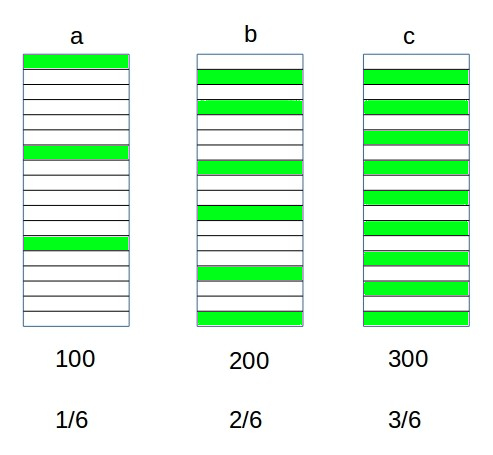
\includegraphics[width=0.5\textwidth]{./imagenes/heuristico/valorSoluciones.jpg}
			\caption{Elección ponderada de candidatos}
			\label{fig: Elección ponderada de candidatos}
		\end{center}
	\end{figure}
	
	\item \textbf{Creación de cola de vuelos extra:} estos vuelos conformarán la cola extra que se añadirá al conjunto de vuelos original, haciendo que éstos tengan mayor posibilidad de ser lanzados antes durante las siguientes \textit{N} iteraciones, tal y como se indica en la fase constructiva:
	
	\item \textbf{Descarte de mala solución} si la mejor de las $N$ soluciones candidatas que se analizan no supera el valor de la mejor solución encontrada hasta el momento, se descarta la cola actual y se reinicia el problema.
	Si se da este caso, indicará que la última cola de candidatos que seleccionamos no ha conseguido mejorar la solución del problema, por tanto podemos descartarla.
\end{enumerate}


\subsection{Parámetros heurístico}
Por tanto el heurístico depende de dos parámetros:
\begin{itemize}
	\item \textbf{$N$}: cada cuantas iteraciones actualizamos la cola de vuelos adicional.
	\item \textbf{$G$}: el tamaño máximo de la cola de vuelos adicionales.
\end{itemize}
Tras realizar pruebas sobre distintos problemas, se ha obtenido que las mejores soluciones se tienen a alcanzar con un parámetro $N$ pequeño y $G$ grande, de forma que la cola de vuelos candidatos sea lo más grande posible y que la fase constructiva se realice con mucha frecuencia. Los resultados se pueden observar en la siguiente sección.

\begin{figure}[H]
	\begin{center}
		\centering
		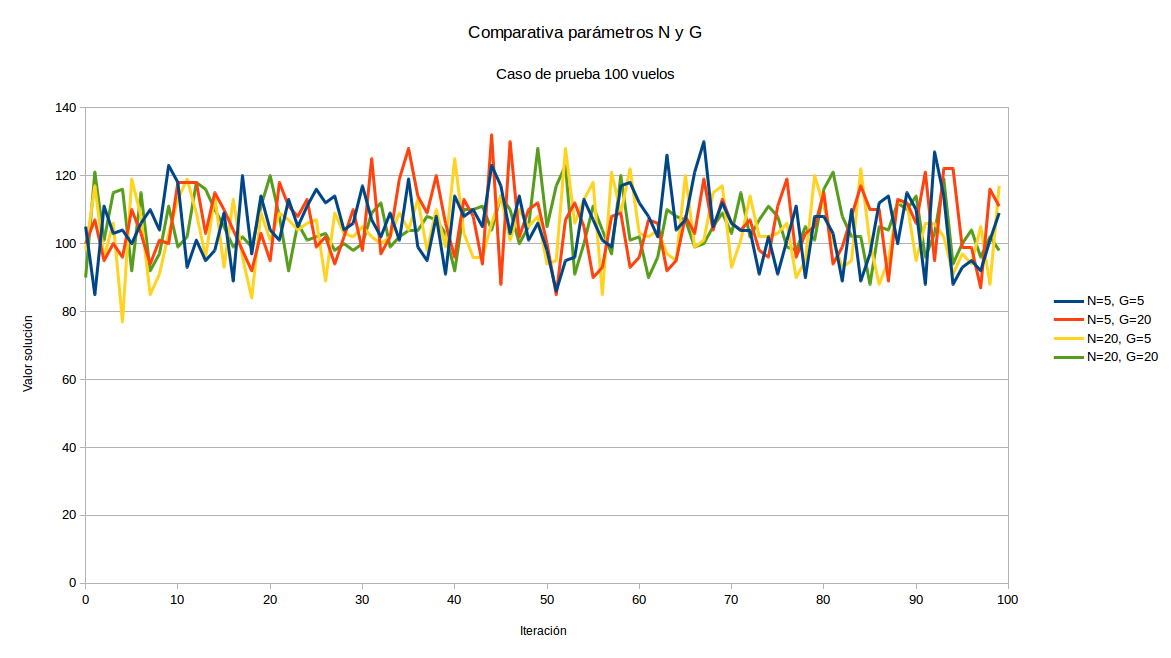
\includegraphics[width=1\textwidth]{./imagenes/heuristico/comparativa_parametros_100_vuelos.png}
		\caption{Comparativa de parámetros G y N}
		\label{fig: Comparativa de parámetros G y N}
	\end{center}
\end{figure}

De esta forma, un alto parámetro $G$ permitirá que muy probablemente muchos de los vuelos que en la mejor solución encontrada hasta ese momento fueron colocados con éxito, se lance, intentando así "reproducir" la mejor solución que se había encontrado. \\
Por contra un bajo parámetro $N$ hará que se cree cada pocas iteraciones una nueva cola de vuelos candidatos, lo que permitirá que en caso de no encontrase rápidamente una solución mejor, se elimine la cola actual y se reinicie el problema.\\
A continuación se muestran los datos obtenidos en una de las simulaciones:



\begin{table}[]
	\centering
	\caption{Comparativa de parámetros $G$ y $N$. Ejemplo problema con 100 vuelos}
	\label{fig: comparativa de parámetros $G$ y $N$. Ejemplo problema con 100 vuelos}
	\begin{tabular}{lllllllllllll}
		& N=2, G=10                                                             & N=2, G=30 & N=2, G=30 &  &  &  &  &  &  &  &  &  \\
		Problema 1 & \multicolumn{1}{c}{\begin{tabular}[c]{@{}c@{}}a\\ b\\ c\end{tabular}} &           &           &  &  &  &  &  &  &  &  &  \\
		Problema 2 &                                                                       &           &           &  &  &  &  &  &  &  &  &  \\
		Problema 3 &                                                                       &           &           &  &  &  &  &  &  &  &  & 
	\end{tabular}
\end{table}


\begin{table}[]
	\centering
	\caption{My caption}
	\label{my-label}
	\begin{tabular}{lllllllllllll}
		\hline
		& N=2, G=10                                                                             & N=2, G=30 & N=2, G=50 & N=5, G=10 & N=5, G=30 & N=5, G=50 & N=10, G=10 & N=10, G=30 & N=10, G=50 & N=20, G=10 & N=20, G=30 & N=20, G=50 \\ \hline
	
		Problema 1 & \multicolumn{1}{c}{\begin{tabular}[c]{@{}c@{}}Máx: 1\\ Med: 2\\ Desv: 3\end{tabular}} &           &           &           &           &           &            &            &            &            &            &            \\
	
		Problema 2 &                                                                                       &           &           &           &           &           &            &            &            &            &            &            \\
		
		Problema 3 &                                                                                       &           &           &           &           &           &            &            &            &            &            &            \\ \hline
	\end{tabular}
\end{table}
Como se puede comprobar, esta combinación de parámetros es la que aporta más aleatoriedad en los resultados, pero es también de media la que aporta mejores resultados, lo que indica que se las malas soluciones son descartadas rápidamente pero se permite explorar un máximo local.


	\chapter{Resultados experimentales}
\label{resultados}

En este capítulo se resumen los resultados obtenidos. Los detalles de los experimentos se pueden consultar en \autoref{anexo1}.

Nota: en todas las pruebas realizadas se ha considerado el escenario más restrictivo posible: la capacidad de un sector en cada instante de tiempo es 1.

\section{Comparación de parámetros $G$ y $N$}
Como se explicó en el \autoref{heurístico}, el algoritmo desarrollado depende de dos parámetros: $G$, la frecuencia con la que realizamos la fase constructiva; y $N$, el número máximo de elementos que puede contener la cola de vuelos extras.

Tras realizar varias pruebas, hemos podido comprobar que, como era de esperar, los mejores resultados se obtienen con un parámetro $N$ pequeño y $G$ grande:
\begin{itemize}
	\item Un \textbf{\textit{N} pequeño} implica realizar la fase constructiva con mucha frecuencia. Esto hace que cada pocas iteraciones busquemos un intento de mejora, y por tanto en caso de no conseguir mejorar la solución actual descartaremos la cola de vuelos extras con mucha rapidez.
	
	Un $N$ pequeño también aporta más desviación a los resultados, ya que al descartar colas con mucha facilidad, hace que el problema se reinicie con más frecuencia, y por tanto tenga más aleatoriedad. 
	
	\item Un \textbf{\textit{G} grande} implica que se de más peso a las buenas soluciones que se localizaron en la cola anterior. Por tanto al tener una cola de vuelos extras de gran tamaño, permite que las buenas soluciones tengan una probabilidad mucho mayor que salir antes en el proceso aleatorio de selección de orden de los vuelos para intentar ser colocados.
\end{itemize} 

Concretamente, hemos podido comprobar mediante pruebas con diferentes parámetros que los la configuración óptima de los parámetros es la siguiente:
\begin{itemize}
	\item \textbf{N:} si es demasiado pequeño, el algoritmo no dispone de las iteraciones suficientes para tratar de obtener información relevante para futuras simulaciones, por lo que el valor óptimo del parámetro es un 5\% del total de iteraciones. De esta forma, en un ejemplo sobre el que realizamos 100 iteraciones, realizaremos la fase constructiva en 20 ocasiones. 
	\item \textbf{G:} aunque el algoritmo funciona mejor con un parámetro \textit{G} elevado, los valores óptimos se alcanzan cuando es un 50\% sobre el número total de vuelos. Por tanto si disponemos de un modelo con 100 vuelos, la cola máxima de vuelos que seleccionaremos para las siguientes iteraciones será de como mucho 50. De esta forma se evita que las iteraciones se parezcan demasiado entre si.
\end{itemize}


\section{Evolución de la función objetivo}
El valor de la función objetivo se obtiene como el sumatorio del valor solución de cada vuelo en el problema:
\begin{equation}\\
\sum valorSolución(f),
\end{equation}
donde cada vuelo $f$ aporta un valor a la solución según la tabla \autoref{table: valores solución}:
\begin{table}[H]
	\centering
	\begin{tabular}{cc}
		\textbf{Estado del vuelo} & \textbf{Valor solución} \\
		Programación inicial      & 5                       \\
		Retrasado                 & 3                       \\
		Desviado                  & 2                       \\
		Retrasado y desviado      & 1                       \\
		Otro caso                 & 0                      
	\end{tabular}
	\caption{Valor solución dependiendo del estado final del vuelo}
	\label{table: valores solución}
\end{table}


Como ya comentamos, con la configuración de parámetros $G$ y $N$ al descartarse muy rápido las malas combinaciones obtenemos un gran número de reseteos del problema, por lo que obtenemos una desviación alta. En la \autoref{fig: Evolucion función objetivo} se muestra la evolución del valor de la función objetivo en un ejemplo de 100 vuelos con parámetro $N=5$: 
\begin{figure}[H]
	\begin{center}
		\centering
		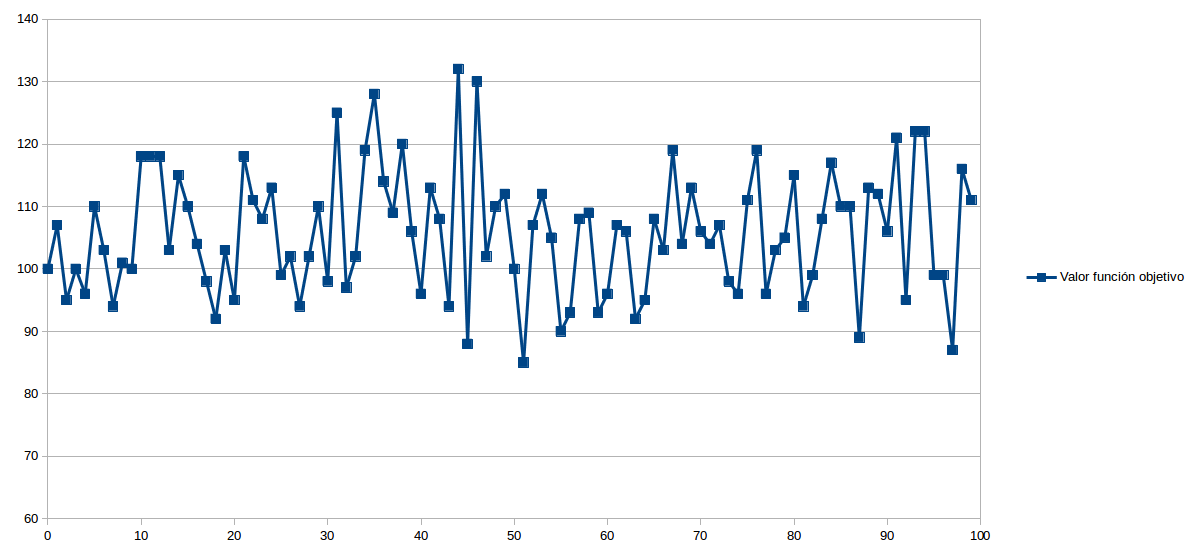
\includegraphics[width=1\textwidth]{./imagenes/resultados/evolucionFuncionObjetivo.png}
		\caption{Evolución función objetivo con $N=5$ y $G=20$ con ejemplo de 100 vuelos}
		\label{fig: Evolucion función objetivo}
	\end{center}
\end{figure}
Como se puede comprobar, en las iteraciones en las que se produce la fase de evaluación y se decide si se descarta la cola, se pueden dar importantes saltos. Por ejemplo, en la \autoref{fig: Evolucion función objetivo} se puede observar como en la iteración con $x=40$ ha habido un descarte de la cola que se había elegido en la anterior fase de mejora, ya que en la siguiente iteración ha habido una gran mejora.

Por el contrario en las iteraciones $x=60$ o $x=80$ se puede observar que no se ha descartado la cola de candidatos, ya que la mejora en la función objetivo ha sido mas leve.

\section{Resultados globales}
A continuación se muestran resumidos los resultados de las pruebas realizadas en los 3 problemas que disponíamos para probar el algoritmo. Los valores se corresponden con la simulación de 100 problemas de 100 iteraciones cada uno con los parámetros $G$ y $N$ óptimos:
\begin{table}[H]
	\centering
	\caption{Resultados pruebas 20 vuelos}
	\label{resultados 20 vuelos}
	\begin{tabular}{lllll}
		& \textbf{\% Vuelos programados} & \textbf{Valor función objetivo} & \textbf{} & \textbf{} \\
		\textbf{Caso A} & \multicolumn{1}{c}{99.61\%} &\multicolumn{1}{c}{46.8} & &\\
		\textbf{Caso B} & \multicolumn{1}{c}{100\% }    &\multicolumn{1}{c}{47} & &\\
		\textbf{Caso C} & \multicolumn{1}{c}{100\%}    &\multicolumn{1}{c}{45} & &
	\end{tabular}
\end{table}


\begin{table}[H]
	\centering
	\caption{Resultados pruebas 100 vuelos}
	\label{resultados 100 vuelos}
	\begin{tabular}{lllll}
		& \textbf{\% Vuelos programados} & \textbf{Valor función objetivo} & \textbf{} & \textbf{} \\
		\textbf{Caso A} & \multicolumn{1}{c}{61.69\%} &\multicolumn{1}{c}{118.57} & &\\
		\textbf{Caso B} & \multicolumn{1}{c}{93.73\%}    &\multicolumn{1}{c}{200.88} & & \\
		\textbf{Caso C} & \multicolumn{1}{c}{99.96\%}    &\multicolumn{1}{c}{217.88} & &
	\end{tabular}
\end{table}

Como se puede observar, exceptuando el caso de pruebas \textit{A} que tiene un gran número de vuelos iguales simultáneos, los resultados se mueven siempre en porcentajes mayores al 90\%.

\section{Representación gráfica}
A continuación se muestra la representación gráfica obtenida para un problema con 20 vuelos.
\begin{figure}[H]
	\begin{center}
		\centering
		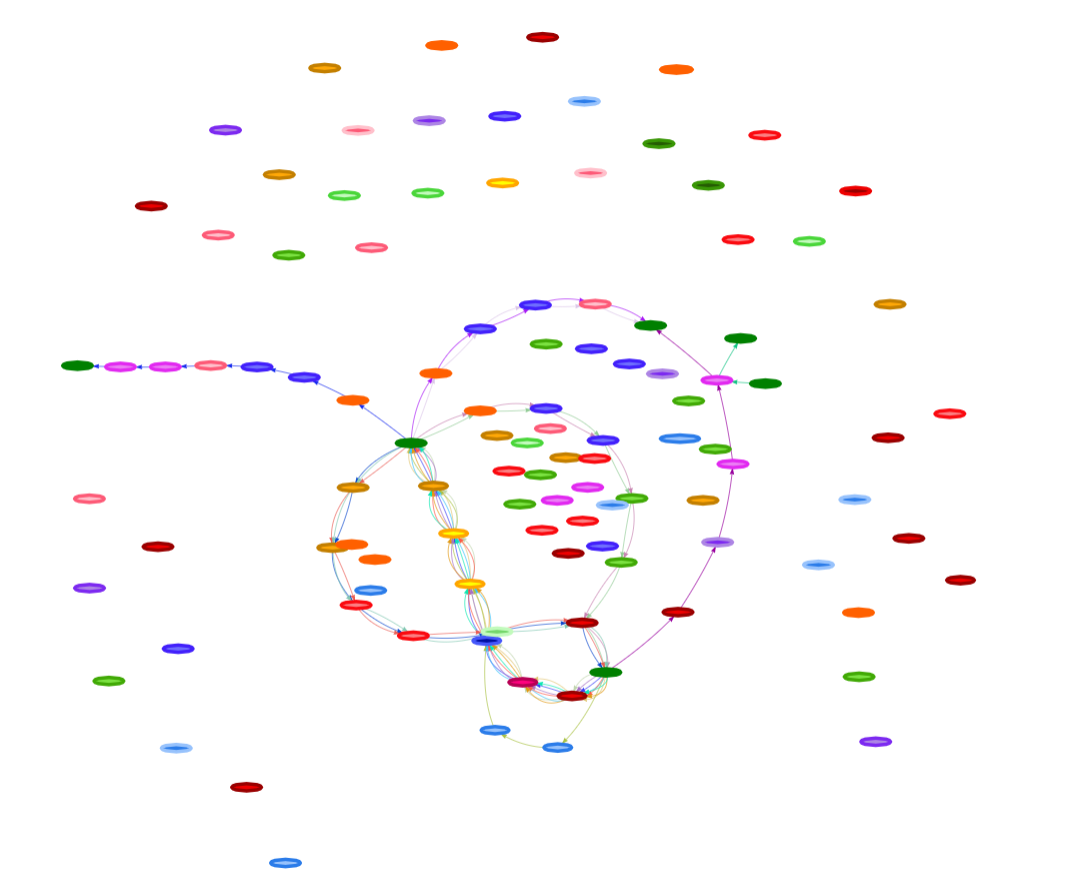
\includegraphics[width=1\textwidth]{./imagenes/resultados/resumenRepresentaion.png}
		\caption{Representación gráfica de un problema de 20 vuelos}
		\label{fig: Representación gráfica de un problema de 20 vuelos}
	\end{center}
\end{figure}

La representación gráfica muestra el resultado final del problema, es decir, se van a representar todos los vuelos a los que se les encontró solución independientemente de los instantes de tiempo en los que estuvieron en tránsito. Por tanto la representación gráfica nos permite observar qué rutas van a ser las más utilizadas.

Algunas características de la representación gráfica:
\begin{itemize}
	\item Sólo muestra los vuelos a los que se les encontró solución.
	\item Los waypoints que están ubicados en el mismo sector se marcan del mismo color (si un waypoint pertenece a más de un sector se escoge solamente el primero para simplificar).
	\item Cada vuelo tiene asignado un color para poder identificar su ruta.
	\item En las aristas del grafo representado se indica el instante de tiempo en el que un vuelo realiza ese trayecto
\end{itemize}

\begin{figure}[H]
	\begin{center}
		\centering
		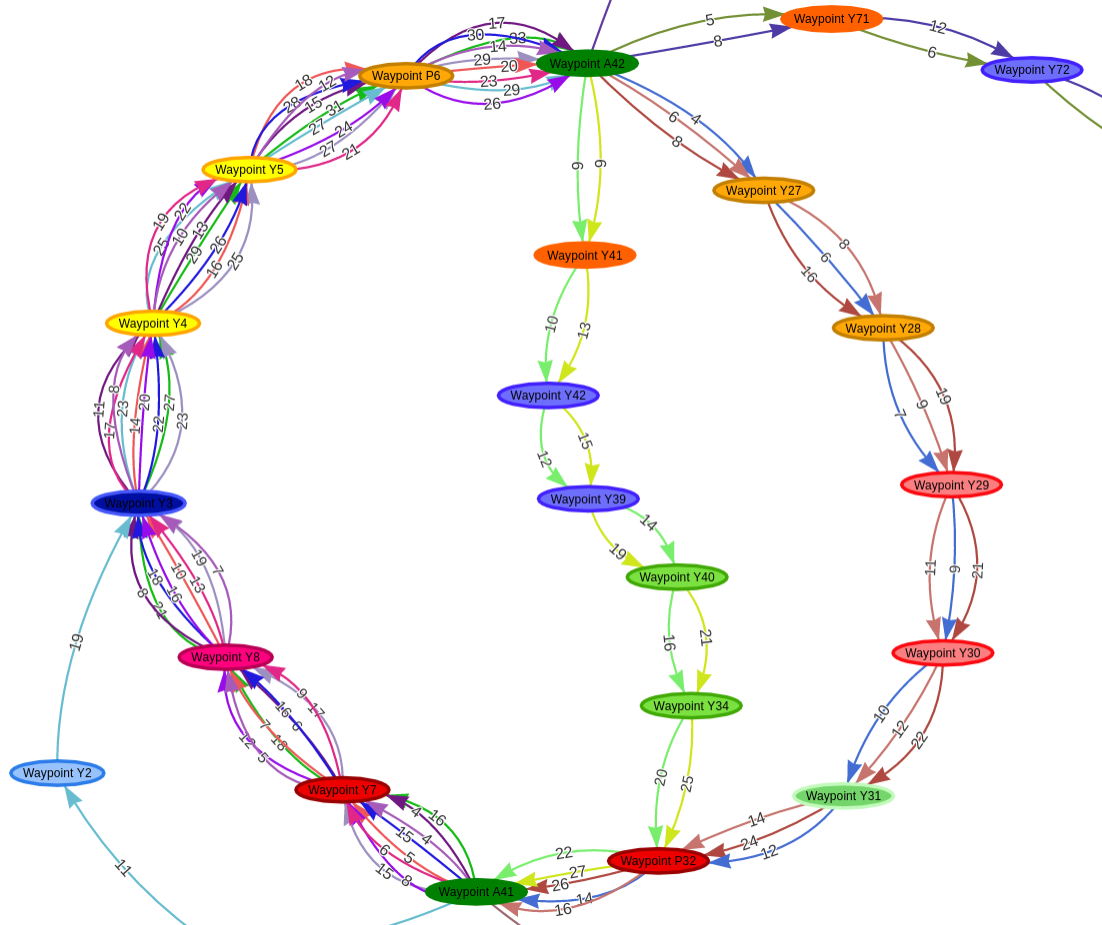
\includegraphics[width=1\textwidth]{./imagenes/resultados/representacionGrafica.png}
		\caption{Ejemplo rutas entre 2 aeropuertos}
		\label{fig: Ejemplo rutas entre 2 aeropuertos}
	\end{center}
\end{figure}

En la \autoref{fig: Ejemplo rutas entre 2 aeropuertos} se puede observar que en el trayecto entre el \textit{Aeropuerto 42} y el \textit{Aeropuerto 41} existen 2 posibles rutas: la rama derecha (más rápida y por tanto con más vuelos) y la rama entral (la ruta alternativa, ya que es más lenta).

\section{Tiempo de ejecución}
Debido al gran volumen de información se maneja el problema, comentamos brevemente el tiempo que equiere el algoritmo. Todas las pruebas han sido realizadas en un Acer Aspire-E5-573G con las siguientes características:
\begin{enumerate}
	\item Sistema operativo Ubuntu 16.04.2 LTS 64-bit.
	\item 8GB de memoria RAM.
	\item Procesador Intel Core i5-4210U CPU 1.70GHz x 4.
	\item tarjeta gráfica GeForce 920M/PCIe/SSE2.
\end{enumerate}

Los tiempos de ejecución en segundos para un problema de $N$ vuelos se resumen en la siguiente tabla y $I$ iteraciones se resumen en la \autoref{tab: Tiempos de ejecución} y en la \autoref{fig: Tiempos de ejecución del programa}:

\begin{table}[h]
	\centering
	\caption{Tiempos de ejecución en segundos }
	\label{tab: Tiempos de ejecución}
	\begin{tabular}{c|l|l|l|}
		\cline{2-4}
		& \multicolumn{1}{c|}{\textbf{N=20}} & \multicolumn{1}{c|}{\textbf{N=100}} & \multicolumn{1}{c|}{\textbf{N=800}} \\ \hline
		\multicolumn{1}{|c|}{\textbf{I=10}} &3  &21  &460  \\ \hline
		\multicolumn{1}{|c|}{\textbf{I=10}} &11  &91  &1363  \\ \hline
		\multicolumn{1}{|c|}{\textbf{I=100}} &74  &680  &9436  \\ \hline
	\end{tabular}
\end{table}


\begin{figure}[]
	\begin{center}
		\centering
		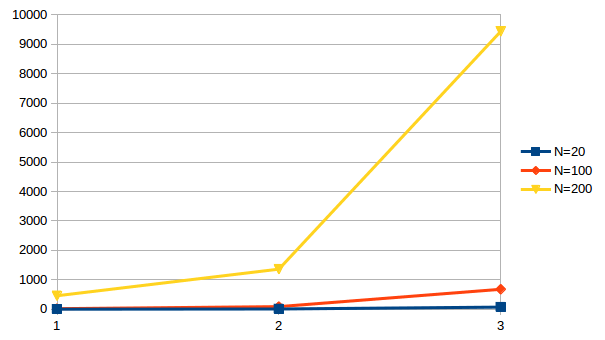
\includegraphics[width=1\textwidth]{./imagenes/resultados/tiemposejecucion.png}
		\caption{Tiempos de ejecución del programa en segundos}
		\label{fig: Tiempos de ejecución del programa}
	\end{center}
\end{figure}

	\section{Conclusiones}
	\chapter{Anexo 1: resultados experimentales}
\label{anexo1}

\section{Comparación parámetros $G$ y $N$}
A continuación se muestran los resultados de las pruebas que hemos realizados variando los parámetros $G$ y $N$ en los tres escenarios de prueba que disponíamos. En la \autoref{tab: comparativa de parámetros $G$ y $N$} se muestran la media de parámetros obtenidos tras realizar 25 experimentos sobre cada caso de prueba.
\begin{figure}[H]
	\begin{center}
		\centering
		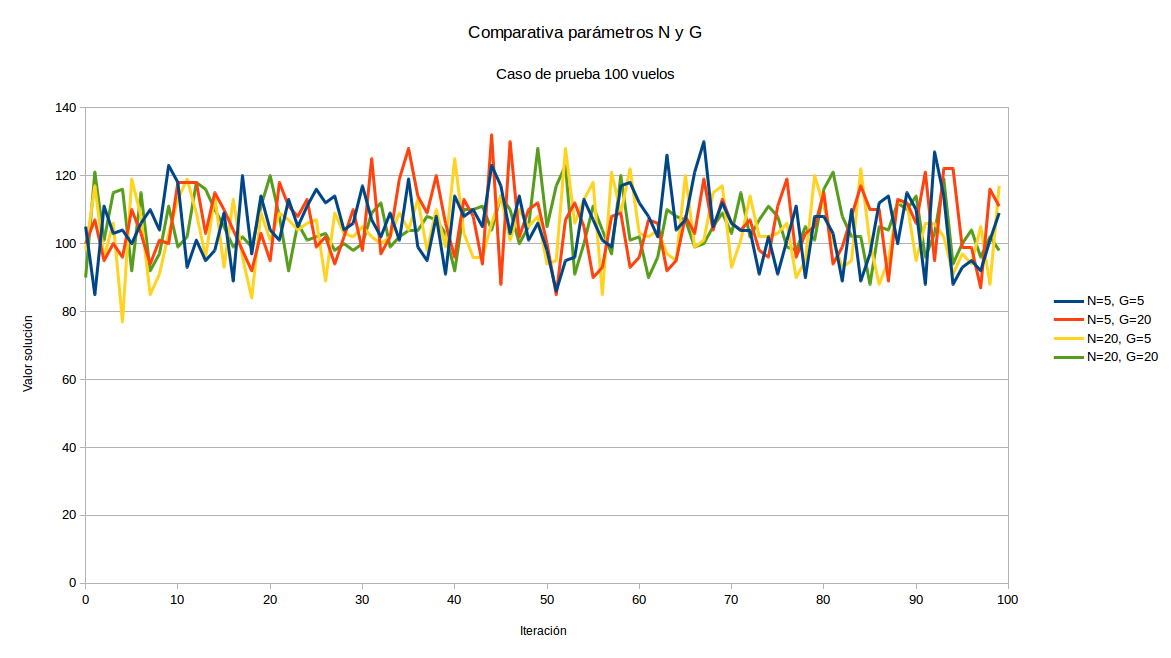
\includegraphics[width=1\textwidth]{./imagenes/heuristico/comparativa_parametros_100_vuelos.png}
		\caption{Evolución función objetivo con diferentes parámetros G y N}
		\label{fig: Evolución función objetivo con diferentes parámetros G y N}
	\end{center}
\end{figure}


\begin{table}[H]
	\centering
	\caption{Comparativa de parámetros $G$ y $N$}
	\label{tab: comparativa de parámetros $G$ y $N$}
	\begin{tabular}{|c|c|c|c|c|}
		\hline
		& \textbf{Problema A} & \textbf{Problema B} & \textbf{Problema C} & \textbf{Media porcentaje éxito} \\ \hline
		\textbf{N=2, G=10} & \% éxito: 64.1 & \% éxito: 94.2 &\% éxito: 99.5 & 85.93\% \\ \hline
		\textbf{N=2, G=30} & \% éxito: 65.2 & \% éxito: 95.1 &\% éxito: 99.5  & 86.60\%\\ \hline
		\textbf{N=2, G=50} & \% éxito: 66.1  & \% éxito: 95.6  &\% éxito: 99.6 & 87.10\%\\ \hline
		\textbf{N=5, G=10} & \% éxito: 65.2  &\textcolor{blue}{\% éxito: 94.3 } &\% éxito: 99.4  &86.30\%\\ \hline
		\textbf{N=5, G=30} & \% éxito: 65.7  &\% éxito: 95.7  &\% éxito: 99.8 &87.06\% \\ \hline
		\textbf{N=5, G=50} & \textcolor{blue}{\% éxito: 66.8} &\% éxito: 95.6  & \textcolor{blue}{\% éxito: 99.8}  &\textcolor{red}{87.40\%} \\ \hline
		\textbf{N=10, G=10} & \% éxito: 64.2  &\% éxito: 94.1  &\% éxito: 99.3  &85.86\% \\  \hline
		\textbf{N=10, G=30} & \% éxito: 65.2  &\% éxito: 95.1  &\% éxito: 99.5  &86.60\% \\ \hline
		\textbf{N=10, G=50} & \% éxito: 65.6  &\% éxito: 95.1  &\% éxito: 99.6  &86.76\% \\ \hline
	\end{tabular}	
\end{table}

Las características de las simulaciones corresponden a las siguientes:
\begin{itemize}
	\item Las pruebas se han realizado sobre los 3 problemas disponibles.
	\item En todos los experimentos se considera el peor escenario: la capacidad de los sectores está limitada a 1.
	\item Se realizan 100 iteraciones sobre cada experimento.
	\item El parámetro $G$
\end{itemize}

\section{Resultados simulación}
\subsection{Caso de pruebas A}
\subsubsection{20 vuelos}
\begin{longtable}{| p{.17\textwidth} | p{.17\textwidth} |  p{.17\textwidth} | p{.17\textwidth}  | p{.17\textwidth} | }
	
	\hline
	\textbf{Iteración} & \textbf{Valor de la función objetivo} &\textbf{\% Vuelos con solución} \\ \hline
	\textbf{0} &46  &100\%  \\ \hline
	\textbf{1} &46  &100\%  \\ \hline
	\textbf{2} &48  &100\%  \\ \hline
	\textbf{3} &47  &100\%  \\ \hline
	\textbf{4} &46  &100\%  \\ \hline
	\textbf{5} &48  &100\%  \\ \hline
	\textbf{6} &48  &100\%  \\ \hline
	\textbf{7} &47  &100\%  \\ \hline
	\textbf{8} &47  &100\%  \\ \hline
	\textbf{9} &46  &100\%  \\ \hline
	\textbf{10} &46  &100\%  \\ \hline
	\textbf{11} &46  &100\%  \\ \hline
	\textbf{12} &46  &100\%  \\ \hline
	\textbf{13} &48  &100\%  \\ \hline
	\textbf{14} &47  &100\%  \\ \hline
	\textbf{15} &47  &100\%  \\ \hline
	\textbf{16} &47  &100\%  \\ \hline
	\textbf{17} &45  &95\%  \\ \hline
	\textbf{18} &47  &100\%  \\ \hline
	\textbf{19} &47  &100\%  \\ \hline
	\textbf{20} &48  &100\%  \\ \hline
	\textbf{21} &45  &95\%  \\ \hline
	\textbf{22} &47  &100\%  \\ \hline
	\textbf{23} &47  &100\%  \\ \hline
	\textbf{24} &47  &100\%  \\ \hline
	\textbf{25} &48  &100\%  \\ \hline
				&Media: \textbf{46.8}  &Media: \textbf{99.61}\%  \\ \hline
	\caption{Resultados problema A 20 vuelos }
	\label{tab: Resultados problema A 20 vuelos}

\end{longtable}




\subsubsection{100 vuelos}

\begin{longtable}{| p{.17\textwidth} | p{.17\textwidth} |  p{.17\textwidth} | p{.17\textwidth}  | p{.17\textwidth} | }
	\hline
	\textbf{Iteración} & \textbf{Valor de la función objetivo} &\textbf{\% Vuelos con solución} \\ \hline
	\textbf{0} &124  &65\%  \\ \hline
	\textbf{1} &112  &61\%  \\ \hline
	\textbf{2} &120  &63\%  \\ \hline
	\textbf{3} &122  &64\%  \\ \hline
	\textbf{4} &122  &62\%  \\ \hline
	\textbf{5} &120  &60\%  \\ \hline
	\textbf{6} &114  &58\%  \\ \hline
	\textbf{7} &116  &62\%  \\ \hline
	\textbf{8} &127  &55\%  \\ \hline
	\textbf{9} &119  &61\%  \\ \hline
	\textbf{10} &121  &63\%  \\ \hline
	\textbf{11} &111  &57\%  \\ \hline
	\textbf{12} &115  &60\%  \\ \hline
	\textbf{13} &114  &58\%  \\ \hline
	\textbf{14} &121  &62\%  \\ \hline
	\textbf{15} &110  &60\%  \\ \hline
	\textbf{16} &119  &61\%  \\ \hline
	\textbf{17} &124  &65\%  \\ \hline
	\textbf{18} &118  &65\%  \\ \hline
	\textbf{19} &112  &60\%  \\ \hline
	\textbf{20} &112  &60\%  \\ \hline
	\textbf{21} &131  &68\%  \\ \hline
	\textbf{22} &116  &60\%  \\ \hline
	\textbf{23} &123  &64\%  \\ \hline
	\textbf{24} &121  &65\%  \\ \hline
	\textbf{25} &119  &61\%  \\ \hline
				&Media: \textbf{118.57}  &Media: \textbf{61.69}\%  \\ \hline

	\caption{Resultados problema A 100 vuelos } % needs to go inside longtable environment
	\label{tab: Resultados problema A 100 vuelos}

	
\end{longtable}





\section{Caso de pruebas B}
\subsubsection{20 vuelos}

\begin{longtable}{| p{.17\textwidth} | p{.17\textwidth} |  p{.17\textwidth} | p{.17\textwidth}  | p{.17\textwidth} | }
	\hline

		\textbf{Iteración} & \textbf{Valor de la función objetivo} &\textbf{\% Vuelos con solución} \\ \hline
		\textbf{0} &47  &100\%  \\ \hline
		\textbf{1} &47  &100\%  \\ \hline
		\textbf{2} &47  &100\%  \\ \hline
		\textbf{3} &47  &100\%  \\ \hline
		\textbf{4} &47  &100\%  \\ \hline
		\textbf{5} &47  &100\%  \\ \hline
		\textbf{6} &47  &100\%  \\ \hline
		\textbf{7} &47  &100\%  \\ \hline
		\textbf{8} &47  &100\%  \\ \hline
		\textbf{9} &47  &100\%  \\ \hline
		\textbf{10} &47  &100\%  \\ \hline
		\textbf{11} &47  &100\%  \\ \hline
		\textbf{12} &47  &100\%  \\ \hline
		\textbf{13} &47  &100\%  \\ \hline
		\textbf{14} &47  &100\%  \\ \hline
		\textbf{15} &47  &100\%  \\ \hline
		\textbf{16} &47  &100\%  \\ \hline
		\textbf{17} &47  &100\%  \\ \hline
		\textbf{18} &47  &100\%  \\ \hline
		\textbf{19} &47  &100\%  \\ \hline
		\textbf{20} &47  &100\%  \\ \hline
		\textbf{21} &47  &100\%  \\ \hline
		\textbf{22} &47  &100\%  \\ \hline
		\textbf{23} &47  &100\%  \\ \hline
		\textbf{24} &47  &100\%  \\ \hline
		\textbf{25} &47  &100\%  \\ \hline
					&Media: \textbf{47}  &Media: \textbf{100}\%  \\ \hline
	\caption{Resultados problema B 20 vuelos } % needs to go inside longtable environment
	\label{tab: Resultados problema B 20 vuelos}

	
\end{longtable}




\subsubsection{100 vuelos}

Resultados del problema 2 con 100 vuelos:
\begin{longtable}{| p{.17\textwidth} | p{.17\textwidth} |  p{.17\textwidth} | p{.17\textwidth}  | p{.17\textwidth} | }
	\hline
	\textbf{Iteración} & \textbf{Valor de la función objetivo} &\textbf{\% Vuelos con solución} \\ \hline
	\textbf{0} &200  &93\%  \\ \hline
	\textbf{1} &202  &96\%  \\ \hline
	\textbf{2} &204  &96\%  \\ \hline
	\textbf{3} &203  &96\%  \\ \hline
	\textbf{4} &203  &95\%  \\ \hline
	\textbf{5} &198  &93\%  \\ \hline
	\textbf{6} &201  &93\%  \\ \hline
	\textbf{7} &201  &94\%  \\ \hline
	\textbf{8} &197  &93\%  \\ \hline
	\textbf{9} &199  &92\%  \\ \hline
	\textbf{10} &199  &93\%  \\ \hline
	\textbf{11} &199  &93\%  \\ \hline
	\textbf{12} &200  &92\%  \\ \hline
	\textbf{13} &199  &93\%  \\ \hline
	\textbf{14} &198  &92\%  \\ \hline
	\textbf{15} &202  &94\%  \\ \hline
	\textbf{16} &205  &96\%  \\ \hline
	\textbf{17} &214  &96\%  \\ \hline
	\textbf{18} &199  &93\%  \\ \hline
	\textbf{19} &202  &96\%  \\ \hline
	\textbf{20} &200  &93\%  \\ \hline
	\textbf{21} &201  &93\%  \\ \hline
	\textbf{22} &200  &93\%  \\ \hline
	\textbf{23} &198  &92\%  \\ \hline
	\textbf{24} &200  &93\%  \\ \hline
	\textbf{25} &199  &93\%  \\ \hline
				&Media: \textbf{200.88}  &Media: \textbf{93.73}\%  \\ \hline
	\caption{Resultados problema B 100 vuelos } 
	\label{tab: Resultados problema B 100 vuelos}

	
\end{longtable}





\subsection{Caso de pruebas C}
\subsubsection{20 vuelos}

Resultados del problema 3 con 20 vuelos:
\begin{longtable}{| p{.17\textwidth} | p{.17\textwidth} |  p{.17\textwidth} | p{.17\textwidth}  | p{.17\textwidth} | }
	\hline
	\textbf{Iteración} & \textbf{Valor de la función objetivo} &\textbf{\% Vuelos con solución} \\ \hline
	\textbf{0} &45 &100\%  \\ \hline
	\textbf{1} &45 &100\%  \\ \hline
	\textbf{2} &45 &100\%  \\ \hline
	\textbf{3} &45 &100\%  \\ \hline
	\textbf{4} &45 &100\%  \\ \hline
	\textbf{5} &45 &100\%  \\ \hline
	\textbf{6} &45 &100\%  \\ \hline
	\textbf{7} &45 &100\%  \\ \hline
	\textbf{8} &45 &100\%  \\ \hline
	\textbf{9} &45 &100\%  \\ \hline
	\textbf{10} &45 &100\%  \\ \hline
	\textbf{11} &45 &100\%  \\ \hline
	\textbf{12} &45 &100\%  \\ \hline
	\textbf{13} &45 &100\%  \\ \hline
	\textbf{14} &45 &100\%  \\ \hline
	\textbf{15} &45 &100\%  \\ \hline
	\textbf{16} &45 &100\%  \\ \hline
	\textbf{17} &45 &100\%  \\ \hline
	\textbf{18} &45 &100\%  \\ \hline
	\textbf{19} &45 &100\%  \\ \hline
	\textbf{20} &45 &100\%  \\ \hline
	\textbf{21} &45 &100\%  \\ \hline
	\textbf{22} &45 &100\%  \\ \hline
	\textbf{23} &45 &100\%  \\ \hline
	\textbf{24} &45 &100\%  \\ \hline
	\textbf{25} &45 &100\%  \\ \hline
				&Media: \textbf{45}  &Media: \textbf{100}\%  \\ \hline
	\caption{Resultados problema C 20 vuelos } % needs to go inside longtable environment
	\label{tab: Resultados problema C 20 vuelos}

	
\end{longtable}



\subsubsection{100 vuelos}

Resultados del problema 3 con 100 vuelos:
\begin{longtable}{| p{.17\textwidth} | p{.17\textwidth} |  p{.17\textwidth} | p{.17\textwidth}  | p{.17\textwidth} | }
	\hline
	\textbf{Iteración} & \textbf{Valor de la función objetivo} &\textbf{\% Vuelos con solución} \\ \hline
	\textbf{0} &218  &100\%  \\ \hline
	\textbf{1} &218  &100\%  \\ \hline
	\textbf{2} &218  &100\%  \\ \hline
	\textbf{3} &218  &100\%  \\ \hline
	\textbf{4} &218  &100\%  \\ \hline
	\textbf{5} &218  &100\%  \\ \hline
	\textbf{6} &218  &100\%  \\ \hline
	\textbf{7} &218  &100\%  \\ \hline
	\textbf{8} &218  &100\%  \\ \hline
	\textbf{9} &218  &100\%  \\ \hline
	\textbf{10} &218  &100\%  \\ \hline
	\textbf{11} &215  &99\%  \\ \hline
	\textbf{12} &218  &100\%  \\ \hline
	\textbf{13} &218  &100\%  \\ \hline
	\textbf{14} &218  &100\%  \\ \hline
	\textbf{15} &218  &100\%  \\ \hline
	\textbf{16} &218  &100\%  \\ \hline
	\textbf{17} &218  &100\%  \\ \hline
	\textbf{18} &218  &100\%  \\ \hline
	\textbf{19} &218  &100\%  \\ \hline
	\textbf{20} &218  &100\%  \\ \hline
	\textbf{21} &218  &100\%  \\ \hline
	\textbf{22} &218  &100\%  \\ \hline
	\textbf{23} &218  &100\%  \\ \hline
	\textbf{24} &218  &100\%  \\ \hline
	\textbf{25} &218  &100\%  \\ \hline
				&Media: \textbf{217.88}  &Media: \textbf{99.96}\%  \\ \hline
	\caption{Resultados problema C 100 vuelos } % needs to go inside longtable environment
	\label{tab: Resultados problema C 100 vuelos}

	
\end{longtable}





	\chapter{Estructura de clases}
\label{anexo2}
Para diseñar la estructura del modelo, se ha creado un esquema de clases cuyas entidades y sus atributos se muestran a continuacion.
\subsection*{Flight}
Es la clase que se encarga de representar a los vuelos en el problema.
\begin{itemize}
	\item \textbf{id}: identificador del vuelo.
	\item \textbf{timeStart}: instante de tiempo en el que el vuelo tiene planeado el despegue.
	\item \textbf{groundDelay}: matriz de costes del grafo de recorridos.
	\item \textbf{routes}: lista de los waypoint route que possee el vuelo.
	\item \textbf{numWaypoint}: número de waypoint que tiene un vuelo.
	\item \textbf{idWaypointStart}: identificador del waypoint en el que se encuentra el aeropuerto de salida.
	\item \textbf{idWaypointEnd}: identificador del waypoint en el que se encuentra el aeropuerto de llegada.
	\item \textbf{status}: estado del vuelo.
	\item \textbf{numRoutes}: número de rutas de las que dispone el vuelo
	\item \textbf{timeFinish}: tiempo de llegada al aeropuerto de destino en su ruta por defecto.
	\item \textbf{waypointnames}: listado de nombres de los waypoints que recorre en todas sus rutas.
	\item \textbf{waypointRoute}: listado de los waypointRoutes que tiene el vuelo
	\item \textbf{numWaypointRoute}: número de waypoint routes que tiene el vuelo.
	\item \textbf{initialSolution}: listado de waypoint route que corresponde a la solución por defecto del vuelo.
	\item \textbf{currentSolution}: solución que tiene el vuelo en cada iteración.
	\item \textbf{flightInterchangeCandidates}: listado de vuelos con sol que el vuelo comparte sectores.
\end{itemize}

\subsection*{Problem}
Representa las características del problema
\begin{itemize}
	\item \textbf{numAirports}: número de aeropuertos que tiene el problema.
	\item \textbf{numSectors}: número de sectores que tiene el problema.
	\item \textbf{numTrajectories}: número de distintas trayectorias que en total tienen todos los vuelos del problema.
	\item \textbf{numWaypoints}: número de waypoints que tiene el problema.
	\item \textbf{numFlights}: número de vuelos que tiene el problema.
	\item \textbf{numTimes}: número de instantes de tiempo que se analizan en el problema.
	\item \textbf{listWaypoints}: listado de los diferentes waypoints de los que se compone el problema.
	\item \textbf{listSectors}: listado de los diferentes sectores de los que se compone el problema.
	\item \textbf{listTimeMoment}: listado de las capacidades y estado de los vuelos en los diferentes instantes de tiempo.
	\item \textbf{listFlights}: listado de los diferentes vuelos de los que se compone el problema.
	\item \textbf{iteration}: iteración en la que se encuentra el problema.
	\item \textbf{log}: documento de teto en el que se guarda un registro de las operaciones que se producen.
	\item \textbf{queueExtraFlights}: cola que contendrá los vuelos seleccionados durante la fase constructiva del algoritmo.
	\item \textbf{solutions}: lista de las diferentes soluciones (estado de cada vuelo y su valor en la función objetivo) obtenidas en cada iteracción.
	\item \textbf{valueBestSolution}: valor de la mejor solución encontrada hasta el momento.
	\item \textbf{routeFlightResults}: ruta del documento en el que se volcarán los datos para su posterior visualización.
\end{itemize}

\subsection*{Sector}
\begin{itemize}
	\item \textbf{id}: identificador del sector.
	\item \textbf{name}: nombre del sector.
	\item \textbf{capacity}: capacidad del sector. En nuestro problema todos los sectores tienen capacidad 1.
\end{itemize}

\subsection*{Solution}
Representa la solución obtenida en cada iteración del problema.
\begin{itemize}
	\item \textbf{flightSolutions}: es un mapa de la forma vuelo => solución del vuelo.
	\item \textbf{value}: valor que tiene la solución. Se obtiene sumando el valor de todos los vuelos de una iteración
\end{itemize}

\subsection*{TimeMoment}
Representa las capacidades del problema para cada instante de tiempo.
\begin{itemize}
	\item \textbf{numFlightMatrix}: es una matriz en la que se indica en que arco de su grafo de recorridos se encuentra cada vuelos. Se utiliza para controlar que no haya 2 vuelos en el mismo instante de tiempo entre 2 waypoints.
	\item \textbf{numFlightsSector}: indica el número de vuelos que hay en cada sector en un momento de tiempo
\end{itemize}

\subsection*{Wapoint}
\begin{itemize}
	\item \textbf{id}: identificador del waypoint.
	\item \textbf{name}: nombre del sector.
	\item \textbf{sectors}: listado de los sectores a los que pertenece el waypoint.
	\item \textbf{isAirport}: booleano que indica si el waypoint es un aeropuerto.
\end{itemize}

\subsection*{WaypointRoute}
Representa a los puntos de ruta que posee cada vuelo. Están formados por un waypoint y un instante de tiempo.
\begin{itemize}
	\item \textbf{id}: identificador del waypointRoute.
	\item \textbf{inTime}: momento de tiempo en el que se da l waypointRoute
\end{itemize}
	\nocite{*}
	\bibliographystyle{bibliografia/apalike-es}
	\bibliography{bibliografia/MyCollection}
	


	
\end{document}